%%%%%%%%%%%%%%%%%%%%%%%%%%%%%%%%%%%%%%%%%%%%%%%%%%%%%%%%%%%%%%%%%%%%%%
%%%%%%%%%%%%%%%%%%%%%%%%%%%%%%%%%%%%%%%%%%%%%%%%%%%%%%%%%%%%%%%%%%%%%%
%%
%% IVT LaTeX template
%%   Kirill Müller
%%   kirill.mueller@ivt.baug.ethz.ch
%%
%%%%%%%%%%%%%%%%%%%%%%%%%%%%%%%%%%%%%%%%%%%%%%%%%%%%%%%%%%%%%%%%%%%%%%
%%%%%%%%%%%%%%%%%%%%%%%%%%%%%%%%%%%%%%%%%%%%%%%%%%%%%%%%%%%%%%%%%%%%%%

%%%%%%%%%%%%%%%%%%%%%%%%%%%%%%%%%%%%%%%%%%%%%%%%%%%%%%%%%%%%%%%%%%%%%%
%%%%%%%%%%%%%%%%%%%%%%%%%%%%%%%%%%%%%%%%%%%%%%%%%%%%%%%%%%%%%%%%%%%%%%
%%
%% Encoding check:
%%   ä  ö  ü  Ä  Ö  Ü  ß  á  é  í  ó  ú  à  è  ì  ò  ù  â  ê  î  ô  û
%%
%%   If the above contains rubbish, please re-open this file using
%%   one of the following encodings: Latin1, ISO-8859-1, Windows-1252.
%%   DO NOT save the file in this case!
%%
%%%%%%%%%%%%%%%%%%%%%%%%%%%%%%%%%%%%%%%%%%%%%%%%%%%%%%%%%%%%%%%%%%%%%%
%%%%%%%%%%%%%%%%%%%%%%%%%%%%%%%%%%%%%%%%%%%%%%%%%%%%%%%%%%%%%%%%%%%%%%

%%%%%%%%%%%%%%%%%%%%%%%%%%%%%%%%%%%%%%%%%%%%%%%%%%%%%%%%%%%%%%%%%%%%%%
%%%%%%%%%%%%%%%%%%%%%%%%%%%%%%%%%%%%%%%%%%%%%%%%%%%%%%%%%%%%%%%%%%%%%%
%%
%% This is an example for writing a paper at the IVT.
%% It supports English and German language.
%% By using it, it is possible to switch paper layouts easily
%% (e.g., working paper style into TRB style)
%%
%% The easiest way to write you own paper is to create an
%% appropriate directory stucture in the papers subdirectory
%% i.e. papers/strc/2007/mypaper,
%% copy this template and modify it there.
%%
%% See the note below on renaming the main file.
%%
%% Each keyword is documented. Just follow the instructions...
%% Enjoy!
%%
%%%%%%%%%%%%%%%%%%%%%%%%%%%%%%%%%%%%%%%%%%%%%%%%%%%%%%%%%%%%%%%%%%%%%%
%%%%%%%%%%%%%%%%%%%%%%%%%%%%%%%%%%%%%%%%%%%%%%%%%%%%%%%%%%%%%%%%%%%%%%

%%%%%%%%%%%%%%%%%%%%%%%%%%%%%%%%%%%%%%%%%%%%%%%%%%%%%%%%%%%%%%%%%%%%%%
%%%%%%%%%%%%%%%%%%%%%%%%%%%%%%%%%%%%%%%%%%%%%%%%%%%%%%%%%%%%%%%%%%%%%%
%%
%% IMPORTANT NOTE ON FILE RENAMES:
%%   If you rename this file, look for the text "Template"
%%   in all files and change this to the new filename, too.
%%   There is a script that will do this for you in
%%   Linux/Windows+cygwin or Mac OS X: Simply execute
%%
%%       _latexfiles/tools/rename.sh Template NewName
%%
%%   Substitute NewName with a name of your choice.
%%
%%   In Windows, use your favorite find-in-text-files tool
%%
%%%%%%%%%%%%%%%%%%%%%%%%%%%%%%%%%%%%%%%%%%%%%%%%%%%%%%%%%%%%%%%%%%%%%%
%%%%%%%%%%%%%%%%%%%%%%%%%%%%%%%%%%%%%%%%%%%%%%%%%%%%%%%%%%%%%%%%%%%%%%

%%%%%%%%%%%%%%%%%%%%%%%%%%%%%%%%%%%%%%%%%%%%%%%%%%%%%%%%%%%%%%%%%%%%%%
%% Location of the common files
%%   If unsure, please leave this as it is
\newcommand{\mypath}{_latexfiles/}
%\newcommand{\mypath}{../../../}
%%%%%%%%%%%%%%%%%%%%%%%%%%%%%%%%%%%%%%%%%%%%%%%%%%%%%%%%%%%%%%%%%%%%%%

%%%%%%%%%%%%%%%%%%%%%%%%%%%%%%%%%%%%%%%%%%%%%%%%%%%%%%%%%%%%%%%%%%%%%%
%% language specification:
%%   Here you define in which langugage your paper will be written.
%%   There are ALWAYS 2 languages to define (even you do not need it.)
%%   Since we are writing only in German or English, other languages
%%   are not supported.
%%   Choose either 'german' or 'english' as your first language.
\newcommand{\myfirstlang}{english}
%%%%%%%%%%%%%%%%%%%%%%%%%%%%%%%%%%%%%%%%%%%%%%%%%%%%%%%%%%%%%%%%%%%%%%

%%%%%%%%%%%%%%%%%%%%%%%%%%%%%%%%%%%%%%%%%%%%%%%%%%%%%%%%%%%%%%%%%%%%%%
%% Include Paper-Layout:
%%   Here the ivt working paper layout is chosen
%%   For changing this paper into i.e. TRB layout just change "ivt-wp"
%%   to "trb"
% !TeX encoding = usascii
% Prepare to get rid of \mypath one day
\providecommand\mypath[3]{}
%%%%%%%%%%%%%%%%%%%%%%%%%%%%%%%%%%%%%%%%%%%%%%%%%%%%%%%%%%%%%%%%%%%%%%
%% $Id: trb-lineNumbered.tex 12326 2013-10-11 10:04:04Z muelleki $
%%%%%%%%%%%%%%%%%%%%%%%%%%%%%%%%%%%%%%%%%%%%%%%%%%%%%%%%%%%%%%%%%%%%%%

%%%%%%%%%%%%%%%%%%%%%%%%%%%%%%%%%%%%%%%%%%%%%%%%%%%%%%%%%%%%%%%%%%%%%%
%%
%% TRB PAPER LAYOUT
%% Date: 2007-06-28
%% author:
%%   Michael Balmer, balmer@ivt.baug.ethz.ch
%%
%%%%%%%%%%%%%%%%%%%%%%%%%%%%%%%%%%%%%%%%%%%%%%%%%%%%%%%%%%%%%%%%%%%%%%

% !TeX encoding = usascii
% Prepare to get rid of \mypath one day
\providecommand\mypath[3]{}
%%%%%%%%%%%%%%%%%%%%%%%%%%%%%%%%%%%%%%%%%%%%%%%%%%%%%%%%%%%%%%%%%%%%%%
%% $Id: trb.tex 17089 2016-08-10 09:29:01Z muelleki $
%%%%%%%%%%%%%%%%%%%%%%%%%%%%%%%%%%%%%%%%%%%%%%%%%%%%%%%%%%%%%%%%%%%%%%

%%%%%%%%%%%%%%%%%%%%%%%%%%%%%%%%%%%%%%%%%%%%%%%%%%%%%%%%%%%%%%%%%%%%%%
%%
%% TRB PAPER LAYOUT
%% Date: 2007-06-28
%% author:
%%   Michael Balmer, balmer@ivt.baug.ethz.ch
%%
%%%%%%%%%%%%%%%%%%%%%%%%%%%%%%%%%%%%%%%%%%%%%%%%%%%%%%%%%%%%%%%%%%%%%%

%%%%%%%%%%%%%%%%%%%%%%%%%%%%%%%%%%%%%%%%%%%%%%%%%%%%%%%%%%%%%%%%%%%%%%
%%%%%%%%%%%%%%%%%%%%%%%%%%%%%%%%%%%%%%%%%%%%%%%%%%%%%%%%%%%%%%%%%%%%%%
%%
%% Standard latex layout configurations
%%   Here, commands and settings are use which are available
%%   by the latex packages
%%
%%%%%%%%%%%%%%%%%%%%%%%%%%%%%%%%%%%%%%%%%%%%%%%%%%%%%%%%%%%%%%%%%%%%%%
%%%%%%%%%%%%%%%%%%%%%%%%%%%%%%%%%%%%%%%%%%%%%%%%%%%%%%%%%%%%%%%%%%%%%%
%% Type of document:
%% - Paperformat: letterpaper, a4paper, a5paper, b5paper,
%%   executivepaper, legalpaper
%% - Main font size: 10pt, 11pt, 12pt
%% - Formulae setting: - (centred), fleqn (left-aligned)
%% - Numbering of formulae: - (right-aligned), leqno (left-aligned)
%% - New page after title: titlepage, notitlepage
%% - Number of columns per page: onecolumn, twocolumn
%% - Page style: oneside, twoside
%% - Paper rotation: - (protrait), landscape
%% - Chapter start: openright, openany (not required for oneside layout)
%% - Mark overfull boxes: draft, final
\documentclass[12pt,fleqn,titlepage,onecolumn,oneside,final]{article}
%%%%%%%%%%%%%%%%%%%%%%%%%%%%%%%%%%%%%%%%%%%%%%%%%%%%%%%%%%%%%%%%%%%%%%
%% borders, margrins and offset
\usepackage[a4paper,left=1.0in,right=1.0in,top=1.0in,bottom=1.0in]{geometry}
%%%%%%%%%%%%%%%%%%%%%%%%%%%%%%%%%%%%%%%%%%%%%%%%%%%%%%%%%%%%%%%%%%%%%%
%% Package options
\PassOptionsToPackage{nooneline,font=bf,labelsep=quad,format=hang}{caption}
\PassOptionsToPackage{font=small,labelsep=space}{subcaption}
\PassOptionsToPackage{fleqn}{amsmath}
\PassOptionsToPackage{compress}{natbib}
\PassOptionsToPackage{noabbrev}{cleveref}
%%%%%%%%%%%%%%%%%%%%%%%%%%%%%%%%%%%%%%%%%%%%%%%%%%%%%%%%%%%%%%%%%%%%%%
%% Include default packages and settings
%%%%%%%%%%%%%%%%%%%%%%%%%%%%%%%%%%%%%%%%%%%%%%%%%%%%%%%%%%%%%%%%%%%%%%
%% Bugfixes:
\ifdefined\ivtnofixltx\else\usepackage{fixltx2e}\fi
%%%%%%%%%%%%%%%%%%%%%%%%%%%%%%%%%%%%%%%%%%%%%%%%%%%%%%%%%%%%%%%%%%%%%%
%% Smart space after macro:
\usepackage{xspace}
%%%%%%%%%%%%%%%%%%%%%%%%%%%%%%%%%%%%%%%%%%%%%%%%%%%%%%%%%%%%%%%%%%%%%%
%% string manipulation
\usepackage{stringstrings}
\usepackage{textcase}
%%%%%%%%%%%%%%%%%%%%%%%%%%%%%%%%%%%%%%%%%%%%%%%%%%%%%%%%%%%%%%%%%%%%%%
%% providing if-then-else command:
\usepackage{ifthen}
%%%%%%%%%%%%%%%%%%%%%%%%%%%%%%%%%%%%%%%%%%%%%%%%%%%%%%%%%%%%%%%%%%%%%%
%% providing expandonce command (and others):
\usepackage{etoolbox}
%%%%%%%%%%%%%%%%%%%%%%%%%%%%%%%%%%%%%%%%%%%%%%%%%%%%%%%%%%%%%%%%%%%%%%
%% LaTeX3 document parsing:
\usepackage{xparse}
%%%%%%%%%%%%%%%%%%%%%%%%%%%%%%%%%%%%%%%%%%%%%%%%%%%%%%%%%%%%%%%%%%%%%%
%% helper commands
\newcommand{\ifeqe}[4]{%
  \ifthenelse{\equal{\expandonce{#1}}{\expandonce{#2}}}{#3}{#4}%
}
\newcommand{\ifeq}[3]{%
  \ifeqe{#1}{#2}{#3}{}%
}
\newcommand{\ifneq}[3]{%
  \ifeqe{#1}{#2}{}{#3}%
}
\newcommand{\ifne}[2]{%
  \ifneq{#1}{}{#2}%
}
%%%%%%%%%%%%%%%%%%%%%%%%%%%%%%%%%%%%%%%%%%%%%%%%%%%%%%%%%%%%%%%%%%%%%%
%% number of words used (wordcount)
%% - include number
\AtBeginDocument{%
\providecommand{\mywordcount}{}%
\renewcommand{\mywordcount}{%
  \newcounter{mywordcount}%
  \IfFileExists{mywordcount}{%
    \input{mywordcount}%
    \setcounter{mywordcount}{\mytextwordcount}%
  }{%
    \newcommand{\mytextwordcount}{Use the script wordcount.py to count}%
  }%
  \newcounter{myequivalentcount}%
  \setcounter{myequivalentcount}{\arabic{mywordcount} + \totvalue{figure} * 250 + \totvalue{table} * 250}%
  \ifthenelse{\equal{\totvalue{table}}{0}}{%
    \newcommand{\mytableid}{}%
  }{%
    \ifthenelse{\equal{\totvalue{table}}{1}}{%
      \newcommand{\mytableid}{ + 1 table}%
    }{%
      \newcommand{\mytableid}{ + \total{table}\xspace tables}%
    }%
  }%
  \ifthenelse{\equal{\totvalue{figure}}{0}}{%
    \newcommand{\myfigureid}{}%
  }{%
    \ifthenelse{\equal{\totvalue{figure}}{1}}{%
      \newcommand{\myfigureid}{ + 1 figure}%
    }{%
      \newcommand{\myfigureid}{ + \total{figure}\xspace figures}%
    }%
  }%
  \ifthenelse{\equal{\arabic{mywordcount}}{\arabic{myequivalentcount}}}{%
    \newcommand{\myeqtext}{}
  }{%
    \newcommand{\myeqtext}{ = \arabic{myequivalentcount} word equivalents}
  }%
  \mytextwordcount\xspace words\myfigureid\mytableid\myeqtext%
}%
}
\newcommand{\ifelsewc}[2]{%
  \ifdefined\wcFileName%
    #1%
  \else%
    #2%
  \fi%
}
\newcommand{\ifwc}[1]{%
  \ifelsewc{#1}{}%
}
\newcommand{\ifnwc}[1]{%
  \ifelsewc{}{#1}%
}
%%%%%%%%%%%%%%%%%%%%%%%%%%%%%%%%%%%%%%%%%%%%%%%%%%%%%%%%%%%%%%%%%%%%%%
%% Support for conversion to Word
\providecommand{\AsPicture}[1]{#1}
\makeatletter
\@ifpackageloaded{tex4ht}{%
  \newcommand{\ifelseht}[2]{#1}%
}{%
  \newcommand{\ifelseht}[2]{#2}%
}%
\makeatother
\newcommand{\ifht}[1]{%
  \ifelseht{#1}{}%
}
\newcommand{\ifnht}[1]{%
  \ifelseht{}{#1}%
}
%%%%%%%%%%%%%%%%%%%%%%%%%%%%%%%%%%%%%%%%%%%%%%%%%%%%%%%%%%%%%%%%%%%%%%
%% Support for make parts of the document (such as page headers)
%% non-selectable
%%   (usually, you also want to ignore these parts when counting
%%    words)
\ifelseht{%
  \DeclareRobustCommand\squelch[1]{#1}%
}{%
  \ifelsewc{%
    \DeclareRobustCommand\squelch[1]{}%
  }{%
    \usepackage{accsupp}
    \DeclareRobustCommand\squelch[1]{%
      \BeginAccSupp{method=plain,ActualText={}}#1\EndAccSupp{}}%
  }
}%
%%%%%%%%%%%%%%%%%%%%%%%%%%%%%%%%%%%%%%%%%%%%%%%%%%%%%%%%%%%%%%%%%%%%%%
%% Table captions aligned with table:
\usepackage{varwidth}
%%%%%%%%%%%%%%%%%%%%%%%%%%%%%%%%%%%%%%%%%%%%%%%%%%%%%%%%%%%%%%%%%%%%%%
%% default language:
\ifthenelse{\equal{\myfirstlang}{german}}{%
  \usepackage[english,german]{babel}%
}{%
  \usepackage[german,english]{babel}%
}
%%%%%%%%%%%%%%%%%%%%%%%%%%%%%%%%%%%%%%%%%%%%%%%%%%%%%%%%%%%%%%%%%%%%%%
%% bibliography:
\usepackage{natbib}
%%%%%%%%%%%%%%%%%%%%%%%%%%%%%%%%%%%%%%%%%%%%%%%%%%%%%%%%%%%%%%%%%%%%%%
%% AMS mathematics:
%%   (include before txfonts, and use txfonts's iint)
\usepackage{amsmath}
\ifnwc{%
  \let\iint\relax
}%
%%%%%%%%%%%%%%%%%%%%%%%%%%%%%%%%%%%%%%%%%%%%%%%%%%%%%%%%%%%%%%%%%%%%%%
%% The package microtype adjusts font width for individual words
%%   in order to achieve better line breaking.
%%   Also, margin kerning makes the margin look more even.
%%   This also renders the use of \sloppy unnecessary.
\usepackage{microtype}
\fussy
%%%%%%%%%%%%%%%%%%%%%%%%%%%%%%%%%%%%%%%%%%%%%%%%%%%%%%%%%%%%%%%%%%%%%%
%% providing umlauts:
\usepackage[utf8]{inputenc}
\ifnwc{%
\usepackage[T1]{fontenc}
}
%%%%%%%%%%%%%%%%%%%%%%%%%%%%%%%%%%%%%%%%%%%%%%%%%%%%%%%%%%%%%%%%%%%%%%
%% line spacing
\ifnwc{%
\usepackage{setspace}
}
%%%%%%%%%%%%%%%%%%%%%%%%%%%%%%%%%%%%%%%%%%%%%%%%%%%%%%%%%%%%%%%%%%%%%%
%% Allow rotating single pages
%% The package is orientated correctly when displayed on screen
\usepackage{pdflscape}
%% Extract command from this package, to be used in the
%% "sidewaysfigure" environment...
\makeatletter
\let\AddPageRotate=\PLS@AddRotate
\let\RemovePageRotate=\PLS@RemoveRotate
\makeatother
%% ...but reset the command that un-rotates pages inside the
%% "landscape" environment, so that the page rotation stays in effect
%% there
%%
%% (AtBeginEnvironment
\ifdefined\AtBeginEnvironment
  \AtBeginEnvironment{landscape}{\def\RemovePageRotate{\relax}}
\else
  \message{Use a recent version of etoolbox package to get
  correct page rotation in the landscape environment.}
\fi
%%%%%%%%%%%%%%%%%%%%%%%%%%%%%%%%%%%%%%%%%%%%%%%%%%%%%%%%%%%%%%%%%%%%%%
%% Hack for orientating sideways{tables,figures} correctly
%%
%% By default, every page is not rotated:
\usepackage{everypage}
\AddEverypageHook{\RemovePageRotate}%
%% The package floatpag implements a hook that is executed
%% when the current float is displayed. We use this hook
%% to add an \AddPageRotate command for the sideways floats.
\usepackage{floatpag}
\ifnwc{%
  \AtBeginDocument{%
    \pagestyle{\mypagestyle}%
    \floatpagestyle{\mypagestyle}%
    \rotfloatpagestyle{\mypagestyle}%
  }
}
\makeatletter
\def\thisfloatcommand#1{%
  \expandafter\expandafter\expandafter\gdef\expandafter\csname\number\@currbox @float\endcsname{#1}\relax}
\makeatother
%%%%%%%%%%%%%%%%%%%%%%%%%%%%%%%%%%%%%%%%%%%%%%%%%%%%%%%%%%%%%%%%%%%%%%
%% Captions and subcaptions
\usepackage{caption}
\ifnht{%
  \usepackage[singlelinecheck=on,labelformat=simple]{subcaption}
  \renewcommand\thesubfigure{(\alph{subfigure})}
  \renewcommand\thesubtable{(\alph{subtable})}
}
%%%%%%%%%%%%%%%%%%%%%%%%%%%%%%%%%%%%%%%%%%%%%%%%%%%%%%%%%%%%%%%%%%%%%%
%% providing graphics:
\usepackage{graphics}
\usepackage{graphicx}
%%%%%%%%%%%%%%%%%%%%%%%%%%%%%%%%%%%%%%%%%%%%%%%%%%%%%%%%%%%%%%%%%%%%%%
%% sideways figures and tables:
\usepackage[figuresright]{rotating}
%%%%%%%%%%%%%%%%%%%%%%%%%%%%%%%%%%%%%%%%%%%%%%%%%%%%%%%%%%%%%%%%%%%%%%
%% figures:
%%   The following are sometimes needed to avoid pushing
%%   the figs to the end of the text.
\def\textfraction{0.0}
\def\topfraction{0.9999}
\def\dbltopfraction{0.9999}
\def\floatpagefraction{0.8}
%%%%%%%%%%%%%%%%%%%%%%%%%%%%%%%%%%%%%%%%%%%%%%%%%%%%%%%%%%%%%%%%%%%%%%
%% tables:
\usepackage{multirow}
%%%%%%%%%%%%%%%%%%%%%%%%%%%%%%%%%%%%%%%%%%%%%%%%%%%%%%%%%%%%%%%%%%%%%%
%% pretty printing:
\usepackage{listings}
%%%%%%%%%%%%%%%%%%%%%%%%%%%%%%%%%%%%%%%%%%%%%%%%%%%%%%%%%%%%%%%%%%%%%%
%% XML code setup:
\lstloadlanguages{XML}
%%
\lstset {
  columns=fullflexible,
  showstringspaces=false,
  basicstyle=\ttfamily\footnotesize,
  lineskip=0pt,
  breaklines=true,
  breakatwhitespace=true,
  breakindent=12pt,
  fontadjust=true,
  keywordstyle=\bfseries,
  commentstyle=\itshape,
  stringstyle=\bfseries\itshape,
  xleftmargin=0mm,
  xrightmargin=0mm,
  tabsize=2
}

\lstdefinelanguage{XML}
{
  morestring=[b]",
  moredelim=[s][\bfseries\color{Maroon}]{<}{\ },
  moredelim=[s][\bfseries\color{Maroon}]{</}{>},
  moredelim=[l][\bfseries\color{Maroon}]{/>},
  moredelim=[l][\bfseries\color{Maroon}]{>},
  morecomment=[s]{<?}{?>},
  morecomment=[s]{<!--}{-->},
  commentstyle=\color{DarkOliveGreen},
  stringstyle=\color{blue},
  identifierstyle=\color{red}
}
%%%%%%%%%%%%%%%%%%%%%%%%%%%%%%%%%%%%%%%%%%%%%%%%%%%%%%%%%%%%%%%%%%%%%%
%% Support for figure and table count:
\usepackage{totcount}
\usepackage{calc}
\regtotcounter{figure}
\regtotcounter{table}
%%%%%%%%%%%%%%%%%%%%%%%%%%%%%%%%%%%%%%%%%%%%%%%%%%%%%%%%%%%%%%%%%%%%%%
%% Less space between enumeration lists
\usepackage{paralist}
\renewenvironment{itemize}[1]{\begin{compactitem}#1}{\end{compactitem}}
\renewenvironment{enumerate}[1]{\begin{compactenum}#1}{\end{compactenum}}
\renewenvironment{description}[0]{\begin{compactdesc}}{\end{compactdesc}}
%%%%%%%%%%%%%%%%%%%%%%%%%%%%%%%%%%%%%%%%%%%%%%%%%%%%%%%%%%%%%%%%%%%%%%
%% Typesetting-quality tables
\usepackage{booktabs}
%%%%%%%%%%%%%%%%%%%%%%%%%%%%%%%%%%%%%%%%%%%%%%%%%%%%%%%%%%%%%%%%%%%%%%
%% new verbatim environment
\usepackage{verbatim}
%%%%%%%%%%%%%%%%%%%%%%%%%%%%%%%%%%%%%%%%%%%%%%%%%%%%%%%%%%%%%%%%%%%%%%
%% Extended color definitions
\PassOptionsToPackage{svgnames}{xcolor}
\usepackage{xcolor}
%%%%%%%%%%%%%%%%%%%%%%%%%%%%%%%%%%%%%%%%%%%%%%%%%%%%%%%%%%%%%%%%%%%%%%
%% Just in case (before hyperref):
\usepackage{float}
\usepackage{longtable}
\usepackage{ltabptch}
\usepackage{nameref}
%%%%%%%%%%%%%%%%%%%%%%%%%%%%%%%%%%%%%%%%%%%%%%%%%%%%%%%%%%%%%%%%%%%%%%
%% Use hyper-refs for URLs and citations,
%% allow line breaks for URLs
%%   include after all other packages, especially after titlesec
\PassOptionsToPackage{obeyspaces}{url}
\ifnht{\usepackage{hyperref}}
\usepackage{url}
%%%%%%%%%%%%%%%%%%%%%%%%%%%%%%%%%%%%%%%%%%%%%%%%%%%%%%%%%%%%%%%%%%%%%%
%% convenient referencing (after hyperref):
\usepackage[capitalize]{cleveref}
%%%%%%%%%%%%%%%%%%%%%%%%%%%%%%%%%%%%%%%%%%%%%%%%%%%%%%%%%%%%%%%%%%%%%%
%% tables (after hyperref):
\usepackage{tabularx}
%%%%%%%%%%%%%%%%%%%%%%%%%%%%%%%%%%%%%%%%%%%%%%%%%%%%%%%%%%%%%%%%%%%%%%
%% do not count words in references
%% count only title, subtitle and abstract, no auxiliary information
\ifwc{%
  \renewcommand{\bibliography}[1]{}%
  \AtBeginDocument{%
    \renewcommand{\createtitlepage}{\mytitle \mysubtitle}%
    \renewcommand{\createabstract}[1]{#1}%
  }%
}
%%%%%%%%%%%%%%%%%%%%%%%%%%%%%%%%%%%%%%%%%%%%%%%%%%%%%%%%%%%%%%%%%%%%%%
%% for document classes that do not provide \captionabove and
%% \captionbelow
\providecommand{\captionabove}[2][]{\caption[#1]{#2}}
\providecommand{\captionbelow}[2][]{\caption[#1]{#2}}

%%%%%%%%%%%%%%%%%%%%%%%%%%%%%%%%%%%%%%%%%%%%%%%%%%%%%%%%%%%%%%%%%%%%%%
%% Header and footer definition:
\usepackage{fancyhdr}%
\newcommand{\mypagestyle}{fancy}
\fancyhf{}%
\fancyhead[R]{\footnotesize \squelch{\nouppercase{\thepage}}}%
\fancyhead[L]{\footnotesize \squelch{\nouppercase{\internauthorstring}}}%
\renewcommand{\headrulewidth}{0pt}%
\renewcommand{\footrulewidth}{0pt}%
%%%%%%%%%%%%%%%%%%%%%%%%%%%%%%%%%%%%%%%%%%%%%%%%%%%%%%%%%%%%%%%%%%%%%%
%% paragraph settings:
\setlength{\parindent}{\parindent}%
\setlength{\parskip}{6pt}
%%%%%%%%%%%%%%%%%%%%%%%%%%%%%%%%%%%%%%%%%%%%%%%%%%%%%%%%%%%%%%%%%%%%%%
%% caption settings:
\DeclareCaptionLabelFormat{allcaps}{\MakeUppercase{#1\ #2}}
\captionsetup*{labelformat=allcaps}
%%%%%%%%%%%%%%%%%%%%%%%%%%%%%%%%%%%%%%%%%%%%%%%%%%%%%%%%%%%%%%%%%%%%%%
%% Define the depth of numbering parts,chapter,sections and paragraphs:
%%   Numbers representing the depth of sectional units:
%%   -1 = \part    (in book or report document classes)
%%    0 = \chapter (in book or report document classes)
%%    0 = \part    (in article document classes)
%%    1 = \section
%%    2 = \subsection
%%    3 = \subsubsection
%%    4 = \paragraph
%%    5 = \subparagraph
\setcounter{secnumdepth}{3}
%%%%%%%%%%%%%%%%%%%%%%%%%%%%%%%%%%%%%%%%%%%%%%%%%%%%%%%%%%%%%%%%%%%%%%
%% citation style:
\setcitestyle{numbers}
\bibpunct{\textit\bgroup(}{)\egroup}{,}{n}{,}{,}
\providecommand{\citenumfont}[1]{}
\renewcommand{\citenumfont}[1]{\textit{#1}}
\renewcommand{\bibnumfmt}[1]{#1.}
\ifthenelse{\equal{\myfirstlang}{german}}{%
  \bibliographystyle{\mypath../_latexfiles/styles/template_ivt-unsrt-ger}%
}{%
  \bibliographystyle{\mypath../_latexfiles/styles/template_ivt-unsrt-eng}%
}
%%%%%%%%%%%%%%%%%%%%%%%%%%%%%%%%%%%%%%%%%%%%%%%%%%%%%%%%%%%%%%%%%%%%%%
%% no indentation for formulae:
\setlength\mathindent{0pt}
%%%%%%%%%%%%%%%%%%%%%%%%%%%%%%%%%%%%%%%%%%%%%%%%%%%%%%%%%%%%%%%%%%%%%%
%% Times font
% !TeX encoding = usascii
%%%%%%%%%%%%%%%%%%%%%%%%%%%%%%%%%%%%%%%%%%%%%%%%%%%%%%%%%%%%%%%%%%%%%%
%% Font:
%% (unfortunately, mathptmx does not provide bold math fonts,
%%  and times still uses the rather different CM font for maths)
\ifnwc{%
  \ifnht{%
    \usepackage{newtxtext}
    \usepackage{newtxmath}
    \usepackage{courier}
    \undef\oct
  }
}


%%%%%%%%%%%%%%%%%%%%%%%%%%%%%%%%%%%%%%%%%%%%%%%%%%%%%%%%%%%%%%%%%%%%%%
%% single line spacing
\singlespacing
%%%%%%%%%%%%%%%%%%%%%%%%%%%%%%%%%%%%%%%%%%%%%%%%%%%%%%%%%%%%%%%%%%%%%%
%% heading settings:
%%   now using the titlesec package
\usepackage{titlesec}
%%
%% legacy (match appearance of previous version)
\newlength{\sectionbeforedist}
\setlength{\sectionbeforedist}{\parskip}
\addtolength{\sectionbeforedist}{1.16ex}
%%
%% section
\titleformat{\section}{\normalfont\bfseries}{}{0pt}{\MakeUppercase}
\titlespacing*{\section}{0in}{\sectionbeforedist}{0.001pt}
%%
%% subsection
\titleformat{\subsection}{\normalfont\bfseries}{}{0pt}{}
\titlespacing*{\subsection}{0in}{\sectionbeforedist}{0.001pt}
%%
%% subsubsection
\titleformat{\subsubsection}{\normalfont\itshape}{}{0pt}{}
\titlespacing*{\subsubsection}{0in}{\sectionbeforedist}{0.001pt}
%%
%% paragraph
\titleformat{\paragraph}[runin]{\normalfont\bfseries}{}{0pt}{}
\titlespacing*{\paragraph}{0in}{\sectionbeforedist}{5pt}
%%
%% subparagraph
\titleformat{\subparagraph}[runin]{\normalfont\itshape}{}{0pt}{}
\titlespacing*{\subparagraph}{0in}{\sectionbeforedist}{5pt}
%%%%%%%%%%%%%%%%%%%%%%%%%%%%%%%%%%%%%%%%%%%%%%%%%%%%%%%%%%%%%%%%%%%%%%

%%%%%%%%%%%%%%%%%%%%%%%%%%%%%%%%%%%%%%%%%%%%%%%%%%%%%%%%%%%%%%%%%%%%%%
%%%%%%%%%%%%%%%%%%%%%%%%%%%%%%%%%%%%%%%%%%%%%%%%%%%%%%%%%%%%%%%%%%%%%%
%% Language-specific words
% !TeX encoding = usascii
%%%%%%%%%%%%%%%%%%%%%%%%%%%%%%%%%%%%%%%%%%%%%%%%%%%%%%%%%%%%%%%%%%%%%%%%%%%%%%%%%%%%%%%%%%%%%%%%%%%%%%%%%%%%%%%%%%%%%%%%%%%%%%%%%%%%%%%%%%%%
%%
%% The following defines language specific words
%%   These are internal commands. They are not used in the main file.
%%   Langugage specific word commands always starts with '\word'
%%
%%%%%%%%%%%%%%%%%%%%%%%%%%%%%%%%%%%%%%%%%%%%%%%%%%%%%%%%%%%%%%%%%%%%%%
%%%%%%%%%%%%%%%%%%%%%%%%%%%%%%%%%%%%%%%%%%%%%%%%%%%%%%%%%%%%%%%%%%%%%%
%% Error message
\newcommand{\langerrmessage}{\errmessage{Wrong language. Define myfirstlang as either english or german.}}
%%%%%%%%%%%%%%%%%%%%%%%%%%%%%%%%%%%%%%%%%%%%%%%%%%%%%%%%%%%%%%%%%%%%%%
%% and/und
\newcommand{\wordand}{\iflanguage{english}{and}{\iflanguage{german}{und}{\langerrmessage}}}
%%%%%%%%%%%%%%%%%%%%%%%%%%%%%%%%%%%%%%%%%%%%%%%%%%%%%%%%%%%%%%%%%%%%%%
%% phone/Tel
\newcommand{\wordphone}{\iflanguage{english}{phone}{\iflanguage{german}{Tel}{\langerrmessage}}}
%%%%%%%%%%%%%%%%%%%%%%%%%%%%%%%%%%%%%%%%%%%%%%%%%%%%%%%%%%%%%%%%%%%%%%
%% fax/Fax
\newcommand{\wordfax}{\iflanguage{english}{fax}{\iflanguage{german}{Fax}{\langerrmessage}}}
%%%%%%%%%%%%%%%%%%%%%%%%%%%%%%%%%%%%%%%%%%%%%%%%%%%%%%%%%%%%%%%%%%%%%%
%% email/EMail
\newcommand{\wordemail}{\iflanguage{english}{email}{\iflanguage{german}{Mail}{\langerrmessage}}}
%%%%%%%%%%%%%%%%%%%%%%%%%%%%%%%%%%%%%%%%%%%%%%%%%%%%%%%%%%%%%%%%%%%%%%
%% Preferred citation style/Bevorzugter Zitierstil
\newcommand{\wordprefcit}{\iflanguage{english}{Preferred citation style}{\iflanguage{german}{Bevorzugter Zitierstil}{\langerrmessage}}}
%%%%%%%%%%%%%%%%%%%%%%%%%%%%%%%%%%%%%%%%%%%%%%%%%%%%%%%%%%%%%%%%%%%%%%
%% Keywords/Schl\"usselw\"orter
\newcommand{\wordkeywords}{\iflanguage{english}{Keywords}{\iflanguage{german}{Schl\"usselw\"orter}{\langerrmessage}}}
%%%%%%%%%%%%%%%%%%%%%%%%%%%%%%%%%%%%%%%%%%%%%%%%%%%%%%%%%%%%%%%%%%%%%%
%% Quelle/Source
\newcommand{\wordsource}{\iflanguage{english}{Source:\ }{\iflanguage{german}{Quelle:\ }{\langerrmessage}}}
%%%%%%%%%%%%%%%%%%%%%%%%%%%%%%%%%%%%%%%%%%%%%%%%%%%%%%%%%%%%%%%%%%%%%%
%% jan,feb,mar,apr,may,jun,jul,aug,sep,oct,nov,dec -> german/english
\newcommand{\wordmonth}{%
  \ifthenelse{\equal{\mymonth}{jan}}{\iflanguage{english}{January}{\iflanguage{german}{Januar}{\langerrmessage}}}%
  {\ifthenelse{\equal{\mymonth}{feb}}{\iflanguage{english}{February}{\iflanguage{german}{Februar}{\langerrmessage}}}%
   {\ifthenelse{\equal{\mymonth}{mar}}{\iflanguage{english}{March}{\iflanguage{german}{M\"arz}{\langerrmessage}}}%
    {\ifthenelse{\equal{\mymonth}{apr}}{\iflanguage{english}{April}{\iflanguage{german}{April}{\langerrmessage}}}%
     {\ifthenelse{\equal{\mymonth}{may}}{\iflanguage{english}{May}{\iflanguage{german}{Mai}{\langerrmessage}}}%
      {\ifthenelse{\equal{\mymonth}{jun}}{\iflanguage{english}{June}{\iflanguage{german}{Juni}{\langerrmessage}}}%
       {\ifthenelse{\equal{\mymonth}{jul}}{\iflanguage{english}{July}{\iflanguage{german}{Juli}{\langerrmessage}}}%
        {\ifthenelse{\equal{\mymonth}{aug}}{\iflanguage{english}{August}{\iflanguage{german}{August}{\langerrmessage}}}%
         {\ifthenelse{\equal{\mymonth}{sep}}{\iflanguage{english}{September}{\iflanguage{german}{September}{\langerrmessage}}}%
          {\ifthenelse{\equal{\mymonth}{oct}}{\iflanguage{english}{October}{\iflanguage{german}{Oktober}{\langerrmessage}}}%
           {\ifthenelse{\equal{\mymonth}{nov}}{\iflanguage{english}{November}{\iflanguage{german}{November}{\langerrmessage}}}%
            {\ifthenelse{\equal{\mymonth}{dec}}{\iflanguage{english}{December}{\iflanguage{german}{Dezember}{\langerrmessage}}}%
             {}}}}}}}}}}}}}
%%%%%%%%%%%%%%%%%%%%%%%%%%%%%%%%%%%%%%%%%%%%%%%%%%%%%%%%%%%%%%%%%%%%%%
%% jan,feb,mar,apr,may,jun,jul,aug,sep,oct,nov,dec -> num
\newcommand{\nummonth}{%
  \ifthenelse{\equal{\mymonth}{jan}}{01}%
  {\ifthenelse{\equal{\mymonth}{feb}}{02}%
   {\ifthenelse{\equal{\mymonth}{mar}}{03}%
    {\ifthenelse{\equal{\mymonth}{apr}}{04}%
     {\ifthenelse{\equal{\mymonth}{may}}{05}%
      {\ifthenelse{\equal{\mymonth}{jun}}{06}%
       {\ifthenelse{\equal{\mymonth}{jul}}{07}%
        {\ifthenelse{\equal{\mymonth}{aug}}{08}%
         {\ifthenelse{\equal{\mymonth}{sep}}{09}%
          {\ifthenelse{\equal{\mymonth}{oct}}{10}%
           {\ifthenelse{\equal{\mymonth}{nov}}{11}%
            {\ifthenelse{\equal{\mymonth}{dec}}{12}%
             {}}}}}}}}}}}}}
%%%%%%%%%%%%%%%%%%%%%%%%%%%%%%%%%%%%%%%%%%%%%%%%%%%%%%%%%%%%%%%%%%%%%%



%%%%%%%%%%%%%%%%%%%%%%%%%%%%%%%%%%%%%%%%%%%%%%%%%%%%%%%%%%%%%%%%%%%%%%
%%%%%%%%%%%%%%%%%%%%%%%%%%%%%%%%%%%%%%%%%%%%%%%%%%%%%%%%%%%%%%%%%%%%%%
%% Internal commands
% !TeX encoding = usascii
%%%%%%%%%%%%%%%%%%%%%%%%%%%%%%%%%%%%%%%%%%%%%%%%%%%%%%%%%%%%%%%%%%%%%%
%%%%%%%%%%%%%%%%%%%%%%%%%%%%%%%%%%%%%%%%%%%%%%%%%%%%%%%%%%%%%%%%%%%%%%
%%
%% The following defines other internal commands
%%   Internal command are not used by the main file.
%%   Internal commands always starts with '\internal'
%%
%%%%%%%%%%%%%%%%%%%%%%%%%%%%%%%%%%%%%%%%%%%%%%%%%%%%%%%%%%%%%%%%%%%%%%
%%%%%%%%%%%%%%%%%%%%%%%%%%%%%%%%%%%%%%%%%%%%%%%%%%%%%%%%%%%%%%%%%%%%%%
%% user defined german keywords/user defined english keywords
%%   The command only returns a string which are defined by the
%%   main file (\mykeywordsEN or \mykeywordsDE)
\newcommand{\internkeywords}{\iflanguage{english}{\mykeywordsEN}{\iflanguage{german}{\mykeywordsDE}{\langerrmessage}}}
%%%%%%%%%%%%%%%%%%%%%%%%%%%%%%%%%%%%%%%%%%%%%%%%%%%%%%%%%%%%%%%%%%%%%%
%% papertype definition
%%   i.e. working paper/Arbeitsberichte Verkehrs- und Raumplanung
%%   i.e. disseration/Doktorarbeit
\providecommand{\internpapertype}{}
%%%%%%%%%%%%%%%%%%%%%%%%%%%%%%%%%%%%%%%%%%%%%%%%%%%%%%%%%%%%%%%%%%%%%%
%% user defined german institution/user defined english institution
%%   The command only returns a string which are defined by the
%%   main file (\myinstitutionEN or \myinstitutionDE)
\newcommand{\interninstitution}{\iflanguage{english}{\myinstitutionEN}{\iflanguage{german}{\myinstitutionDE}{\langerrmessage}}}
%%%%%%%%%%%%%%%%%%%%%%%%%%%%%%%%%%%%%%%%%%%%%%%%%%%%%%%%%%%%%%%%%%%%%%
%% authorlist
%%   prints out all the given author in a specified way
\newcommand{\internauthorlist}{%
  \providecommand{\myseventhauthor}{}%
  \providecommand{\myeighthauthor}{}%
  \providecommand{\myninthauthor}{}%
  \providecommand{\mytenthauthor}{}%
  \providecommand{\myeleventhauthor}{}%
  \providecommand{\mytwelfthauthor}{}%
  \ifthenelse{\equal{\myseventhauthor}{}}{%
  \ifthenelse{\equal{\myfirstauthor}{}}{}{\myfirstauthor}%
  \ifthenelse{\equal{\mysecondauthor}{}}{}{\newline\mysecondauthor}%
  \ifthenelse{\equal{\mythirdauthor}{}}{}{\newline\mythirdauthor}%
  \ifthenelse{\equal{\myfourthauthor}{}}{}{\newline\myfourthauthor}%
  \ifthenelse{\equal{\myfifthauthor}{}}{}{\newline\myfifthauthor}%
  \ifthenelse{\equal{\mysixthauthor}{}}{}{\newline\mysixthauthor}%
  }%
  {%
  \begin{tabular}{@{}ll@{}}
  \myfirstauthor & \mysecondauthor \\
  \mythirdauthor & \myfourthauthor \\
  \myfifthauthor & \mysixthauthor \\
  \myseventhauthor & \myeighthauthor \\
  \myninthauthor & \mytenthauthor \\
  \myeleventhauthor & \mytwelfthauthor \\
  \end{tabular}%
  }%
}
%%%%%%%%%%%%%%%%%%%%%%%%%%%%%%%%%%%%%%%%%%%%%%%%%%%%%%%%%%%%%%%%%%%%%%
%% author names as a single line
\newcommand{\internauthorstringlong}{%
  \providecommand{\myseventhauthor}{}%
  \providecommand{\myeighthauthor}{}%
  \providecommand{\myninthauthor}{}%
  \providecommand{\mytenthauthor}{}%
  \providecommand{\myeleventhauthor}{}%
  \providecommand{\mytwelfthauthor}{}%
  \ifthenelse{\equal{\myfirstauthor}{}}{}{%
    \myfirstauthor%
    \ifthenelse{\equal{\mysecondauthor}{}}{}{%
      \ifthenelse{\equal{\mythirdauthor}{}}{\ \wordand}{,}
      \mysecondauthor%
      \ifthenelse{\equal{\mythirdauthor}{}}{}{%
        \ifthenelse{\equal{\myfourthauthor}{}}{\ \wordand}{,}
        \mythirdauthor%
        \ifthenelse{\equal{\myfourthauthor}{}}{}{%
          \ifthenelse{\equal{\myfifthauthor}{}}{\ \wordand}{,}
          \myfourthauthor%
          \ifthenelse{\equal{\myfifthauthor}{}}{}{%
            \ifthenelse{\equal{\mysixthauthor}{}}{\ \wordand}{,}
            \myfifthauthor%
            \ifthenelse{\equal{\mysixthauthor}{}}{}{%
              \ifthenelse{\equal{\myseventhauthor}{}}{\ \wordand}{,}
              \mysixthauthor%
              \ifthenelse{\equal{\myseventhauthor}{}}{}{%
                \ifthenelse{\equal{\myeighthauthor}{}}{\ \wordand}{,}
                \myseventhauthor%
                \ifthenelse{\equal{\myeighthauthor}{}}{}{%
                  \ifthenelse{\equal{\myninthauthor}{}}{\ \wordand}{,}
                  \myeighthauthor%
                  \ifthenelse{\equal{\myninthauthor}{}}{}{%
                    \ifthenelse{\equal{\mytenthauthor}{}}{\ \wordand}{,}
                    \myninthauthor%
                    \ifthenelse{\equal{\mytenthauthor}{}}{}{%
                      \ifthenelse{\equal{\myeleventhauthor}{}}{\ \wordand}{,}
                      \mytenthauthor%
                      \ifthenelse{\equal{\myeleventhauthor}{}}{}{%
                        \ifthenelse{\equal{\mytwelfthauthor}{}}{\ \wordand}{,}
                        \myeleventhauthor%
                        \ifthenelse{\equal{\mytwelfthauthor}{}}{}{%
                          \ifthenelse{\equal{}{}}{\ \wordand}{,}
                          \mytwelfthauthor%
                        }%
                      }%
                    }%
                  }%
                }%
              }%
            }%
          }%
        }%
      }%
    }%
  }%
  \ 
}
%%%%%%%%%%%%%%%%%%%%%%%%%%%%%%%%%%%%%%%%%%%%%%%%%%%%%%%%%%%%%%%%%%%%%%
%% author names as a single line, abbreviated
\newcommand{\internauthorstring}{%
  \providecommand{\myseventhauthorREF}{}%
  \providecommand{\myeighthauthorREF}{}%
  \providecommand{\myninthauthorREF}{}%
  \providecommand{\mytenthauthorREF}{}%
  \providecommand{\myeleventhauthorREF}{}%
  \providecommand{\mytwelfthauthorREF}{}%
  \ifthenelse{\equal{\myfirstauthorREF}{}}{}{%
    \myfirstauthorREF%
    \ifthenelse{\equal{\mysecondauthorREF}{}}{}{%
      \ifthenelse{\equal{\mythirdauthorREF}{}}{\ \wordand}{,}
      \mysecondauthorREF%
      \ifthenelse{\equal{\mythirdauthorREF}{}}{}{%
        \ifthenelse{\equal{\myfourthauthorREF}{}}{\ \wordand}{,}
        \mythirdauthorREF%
        \ifthenelse{\equal{\myfourthauthorREF}{}}{}{%
          \ifthenelse{\equal{\myfifthauthorREF}{}}{\ \wordand}{,}
          \myfourthauthorREF%
          \ifthenelse{\equal{\myfifthauthorREF}{}}{}{%
            \ifthenelse{\equal{\mysixthauthorREF}{}}{\ \wordand}{,}
            \myfifthauthorREF%
            \ifthenelse{\equal{\mysixthauthorREF}{}}{}{%
              \ifthenelse{\equal{\myseventhauthorREF}{}}{\ \wordand}{,}
              \mysixthauthorREF%
              \ifthenelse{\equal{\myseventhauthorREF}{}}{}{%
                \ifthenelse{\equal{\myeighthauthorREF}{}}{\ \wordand}{,}
                \myseventhauthorREF%
                \ifthenelse{\equal{\myeighthauthorREF}{}}{}{%
                  \ifthenelse{\equal{\myninthauthorREF}{}}{\ \wordand}{,}
                  \myeighthauthorREF%
                  \ifthenelse{\equal{\myninthauthorREF}{}}{}{%
                    \ifthenelse{\equal{\mytenthauthorREF}{}}{\ \wordand}{,}
                    \myninthauthorREF%
                    \ifthenelse{\equal{\mytenthauthorREF}{}}{}{%
                      \ifthenelse{\equal{\myeleventhauthorREF}{}}{\ \wordand}{,}
                      \mytenthauthorREF%
                      \ifthenelse{\equal{\myeleventhauthorREF}{}}{}{%
                        \ifthenelse{\equal{\mytwelfthauthorREF}{}}{\ \wordand}{,}
                        \myeleventhauthorREF%
                        \ifthenelse{\equal{\mytwelfthauthorREF}{}}{}{%
                          \ifthenelse{\equal{}{}}{\ \wordand}{,}
                          \mytwelfthauthorREF%
                        }%
                      }%
                    }%
                  }%
                }%
              }%
            }%
          }%
        }%
      }%
    }%
  }%
  \ 
}
%%%%%%%%%%%%%%%%%%%%%%%%%%%%%%%%%%%%%%%%%%%%%%%%%%%%%%%%%%%%%%%%%%%%%%
%% author names with address references (used in HKSTS)
\newcommand{\internauthortitlestring}{%
  \ifthenelse{\equal{\mysecondauthor}{}}{%
    \myfirstauthor$^\myfirstauthoraddress$\ %
  }{%
    \ifthenelse{\equal{\mythirdauthor}{}}{%
      \myfirstauthor$^\myfirstauthoraddress$\ \wordand\ \mysecondauthor$^\mysecondauthoraddress$\ %
    }{%
      \ifthenelse{\equal{\myfourthauthor}{}}{%
        \myfirstauthor$^\myfirstauthoraddress$, \mysecondauthor$^\mysecondauthoraddress$\ \wordand\ \mythirdauthor$^\mythirdauthoraddress$\ %
      }{%
        \ifthenelse{\equal{\myfifthauthor}{}}{%
          \myfirstauthor$^\myfirstauthoraddress$, \mysecondauthor$^\mysecondauthoraddress$, \mythirdauthor$^\mythirdauthoraddress$\ \wordand\ \myfourthauthor$^\myfourthauthoraddress$\ %
        }{%
          \ifthenelse{\equal{\mysixthauthor}{}}{%
            \myfirstauthor$^\myfirstauthoraddress$, \mysecondauthor$^\mysecondauthoraddress$, \mythirdauthor$^\mythirdauthoraddress$, \myfourthauthor$^\myfourthauthoraddress$\ \wordand\ \myfifthauthor$^\myfifthauthoraddress$\ %
          }{%
            \myfirstauthor$^\myfirstauthoraddress$, \mysecondauthor$^\mysecondauthoraddress$, \mythirdauthor$^\mythirdauthoraddress$, \myfourthauthor$^\myfourthauthoraddress$, \myfifthauthor$^\myfifthauthoraddress$\ \wordand\ \mysixthauthor$^\mysixthauthoraddress$\ %
          }%
        }%
      }%
    }%
  }%
}
%%%%%%%%%%%%%%%%%%%%%%%%%%%%%%%%%%%%%%%%%%%%%%%%%%%%%%%%%%%%%%%%%%%%%%
%% address list compatible with \internauthortitlestring
\newcommand{\internaddresslist}{%
  \ifne\mysecondaddress{$^a$}%
  \myfirstaddress\\%
  \ifne\mysecondaddress{%
    $^b$\mysecondaddress\\%
      \ifne\mythirdaddress{%
        $^c$\mythirdaddress\\%
          \ifne\myfourthaddress{%
            $^d$\myfourthaddress\\%
              \ifne\myfifthaddress{%
                $^e$\myfifthaddress\\%
                  \ifne\mysixthaddress{%
                    $^f$\mysixthaddress\\%
  }}}}}%
}
%%%%%%%%%%%%%%%%%%%%%%%%%%%%%%%%%%%%%%%%%%%%%%%%%%%%%%%%%%%%%%%%%%%%%%
%% \internmakeonecolumn{entry1}
%%   creates a table with one column containing the given entries
\AtBeginDocument{%
  \newlength{\interncolumnwidth}%
}
\newcommand{\internmakeonecolumn}[1]{{%
  \settowidth{\interncolumnwidth}{#1}%
  \ifthenelse{\lengthtest{\interncolumnwidth=0pt}}{}{%
    #1\\
  }%
}}
%%%%%%%%%%%%%%%%%%%%%%%%%%%%%%%%%%%%%%%%%%%%%%%%%%%%%%%%%%%%%%%%%%%%%%
%% \internmaketwocolumns{entry1}{entry2}
%%   creates a table with two columns containing the given entries
\newcommand{\internmaketwocolumns}[2]{
  \settowidth{\interncolumnwidth}{#1}%
  \ifthenelse{\lengthtest{\interncolumnwidth=0pt}}{}{%
    #1\hfill{}#2\\
  }%
}
%%%%%%%%%%%%%%%%%%%%%%%%%%%%%%%%%%%%%%%%%%%%%%%%%%%%%%%%%%%%%%%%%%%%%%
%% \internmakethreecolumns{entry1}{entry2}{entry3}
%%   creates a table with three columns containing the given entries
\newcommand{\internmakethreecolumns}[3]{
  \settowidth{\interncolumnwidth}{#1}%
  \ifthenelse{\lengthtest{\interncolumnwidth=0pt}}{}{%
    #1\hfill{}#2\hfill{}#3\\
  }%
}
%%%%%%%%%%%%%%%%%%%%%%%%%%%%%%%%%%%%%%%%%%%%%%%%%%%%%%%%%%%%%%%%%%%%%%
%% citation
%%   returns the language specific citation of the paper
%%   default: no citation
\providecommand{\interncitation}{}
%%%%%%%%%%%%%%%%%%%%%%%%%%%%%%%%%%%%%%%%%%%%%%%%%%%%%%%%%%%%%%%%%%%%%%

%%%%%%%%%%%%%%%%%%%%%%%%%%%%%%%%%%%%%%%%%%%%%%%%%%%%%%%%%%%%%%%%%%%%%%
%%%%%%%%%%%%%%%%%%%%%%%%%%%%%%%%%%%%%%%%%%%%%%%%%%%%%%%%%%%%%%%%%%%%%%
%%
%% Standard commands
%%   The following commands >>>HAVE<<< to be defined, because
%%   they are called by the main file.
%%   Standard commands always starts with '\create'. (except
%%   '\switchlanguage' since it would sound stupid ^_^ and
%%   '\ackname' since it is the standard def in babel the package)
%%
%%%%%%%%%%%%%%%%%%%%%%%%%%%%%%%%%%%%%%%%%%%%%%%%%%%%%%%%%%%%%%%%%%%%%%
%% switch language
\newcommand{\switchlanguage}{\iflanguage{english}{\selectlanguage{german}}{\selectlanguage{english}}}
%%%%%%%%%%%%%%%%%%%%%%%%%%%%%%%%%%%%%%%%%%%%%%%%%%%%%%%%%%%%%%%%%%%%%%
%% switch language
\newcommand{\ackname}{\iflanguage{english}{Acknowledgement}{\iflanguage{german}{Danksagung}{\langerrmessage}}}

%%%%%%%%%%%%%%%%%%%%%%%%%%%%%%%%%%%%%%%%%%%%%%%%%%%%%%%%%%%%%%%%%%%%%%
%% PDF keywords
%%%%%%%%%%%%%%%%%%%%%%%%%%%%%%%%%%%%%%%%%%%%%%%%%%%%%%%%%%%%%%%%%%%%%%
\AtBeginDocument{
  \ifthenelse{\equal{\mysecondauthor}{}}{%
    \newcommand{\internpdfauthorstring}{%
      \myfirstauthor%
    }
  }{%
    \ifthenelse{\equal{\mythirdauthor}{}}{%
      \newcommand{\internpdfauthorstring}{%
        \myfirstauthor, \mysecondauthor%
      }
    }{%
      \ifthenelse{\equal{\myfourthauthor}{}}{%
        \newcommand{\internpdfauthorstring}{%
          \myfirstauthor, \mysecondauthor, \mythirdauthor%
        }
      }{%
        \ifthenelse{\equal{\myfifthauthor}{}}{%
          \newcommand{\internpdfauthorstring}{%
            \myfirstauthor, \mysecondauthor, \mythirdauthor, \myfourthauthor%
          }
        }{%
          \ifthenelse{\equal{\mysixthauthor}{}}{%
            \newcommand{\internpdfauthorstring}{%
              \myfirstauthor, \mysecondauthor, \mythirdauthor, \myfourthauthor, \myfifthauthor%
            }
          }{%
            \newcommand{\internpdfauthorstring}{%
              \myfirstauthor, \mysecondauthor, \mythirdauthor, \myfourthauthor, \myfifthauthor, \mysixthauthor%
            }
          }%
        }%
      }%
    }%
  }%
  \providecommand{\mysubject}{}
  \ifnht{%
    \hypersetup{
      pdfauthor={\internpdfauthorstring},
      pdftitle={\mytitle},
      pdfsubject={\mysubject},
      pdfkeywords={\mykeywordsEN}
    }%
  }
}

%%%%%%%%%%%%%%%%%%%%%%%%%%%%%%%%%%%%%%%%%%%%%%%%%%%%%%%%%%%%%%%%%%%%%%
%%%%%%%%%%%%%%%%%%%%%%%%%%%%%%%%%%%%%%%%%%%%%%%%%%%%%%%%%%%%%%%%%%%%%%
%% Hyperlink color
% !TeX encoding = usascii
\ifnht{%
    \hypersetup{
        citebordercolor=ForestGreen,
        linkbordercolor=Crimson,
        urlbordercolor=blue,
        pdfborder={0 0 0.35 [1 2]},
        plainpages=false
    }
}

%%%%%%%%%%%%%%%%%%%%%%%%%%%%%%%%%%%%%%%%%%%%%%%%%%%%%%%%%%%%%%%%%%%%%%
%%%%%%%%%%%%%%%%%%%%%%%%%%%%%%%%%%%%%%%%%%%%%%%%%%%%%%%%%%%%%%%%%%%%%%
%% Figure definitions
% !TeX encoding = usascii
%%%%%%%%%%%%%%%%%%%%%%%%%%%%%%%%%%%%%%%%%%%%%%%%%%%%%%%%%%%%%%%%%%%%%%
%% Caption on top or at bottom?
%%   TRB guidelines: Caption at bottom
\providecommand{\figurecaptionandcontents}[2]{#2#1}
%%%%%%%%%%%%%%%%%%%%%%%%%%%%%%%%%%%%%%%%%%%%%%%%%%%%%%%%%%%%%%%%%%%%%%
%% Caption on top or at bottom for tables?
%%   TRB guidelines: Caption at top
\providecommand{\tablecaptionandcontents}[2]{#1#2}
%%%%%%%%%%%%%%%%%%%%%%%%%%%%%%%%%%%%%%%%%%%%%%%%%%%%%%%%%%%%%%%%%%%%%%
%% Use hrules?
%%   No
\newcommand{\figurerule}{}
\providecommand{\figurecontentsafter}{\end{\figurecontentsenv}\vspace{-2ex}}
%%%%%%%%%%%%%%%%%%%%%%%%%%%%%%%%%%%%%%%%%%%%%%%%%%%%%%%%%%%%%%%%%%%%%%
%% Input definition file
\input{\mypath../_latexfiles/_layouts/_figure}

%%%%%%%%%%%%%%%%%%%%%%%%%%%%%%%%%%%%%%%%%%%%%%%%%%%%%%%%%%%%%%%%%%%%%%

%%%%%%%%%%%%%%%%%%%%%%%%%%%%%%%%%%%%%%%%%%%%%%%%%%%%%%%%%%%%%%%%%%%%%%
%% Contact
%%   \createcontact
%%     {<Name>}
%%     {<andreas line 1>}
%%     {<andreas line 1>}
%%     {<andreas line 3>}
%%     {<phone number>}
%%     {<fax number>}
%%     {<email address>}
\newcommand{\createcontact}[7]{
  \ifthenelse{\equal{#1}{}}{%
    \parbox[t][][l]{\textwidth}{
    }%
  }{%
    \parbox[t][][l]{\textwidth}{
      \raggedright%
      \singlespacing%
      #1\par
      #2, #3, #4\par
      \ifne{#5}{\wordphone: #5\par}
      \ifne{#6}{\wordfax: #6\par}
      #7\par
    }%
  }%
}
%%%%%%%%%%%%%%%%%%%%%%%%%%%%%%%%%%%%%%%%%%%%%%%%%%%%%%%%%%%%%%%%%%%%%%
%% Titlepage definition
\newcommand{\createtitlepage}{
  \begin{titlepage}
    \setcounter{page}{0}
    \setlength\parindent{0pt}%
    \raggedright%
    \textbf{\mytitle}

    \vspace{0.1in}

    Date of submission: \myyear-\nummonth-\myday

    \vspace{0.1in}

    \ifthenelse{\equal{\myfirstauthor}{}}{}{\myfirstaddress}

    \ifthenelse{\equal{\mysecondauthor}{}}{}{\mysecondaddress}

    \ifthenelse{\equal{\mythirdauthor}{}}{}{\mythirdaddress}

    \ifthenelse{\equal{\myfourthauthor}{}}{}{\myfourthaddress}

    \ifthenelse{\equal{\myfifthauthor}{}}{}{\myfifthaddress}

    \ifthenelse{\equal{\mysixthauthor}{}}{}{\mysixthaddress}

    \ifthenelse{\equal{\myseventhauthor}{}}{}{\myseventhaddress}

    \vspace{0.1in}

    Words: \mywordcount

    \vfill
  \end{titlepage}
}
%%%%%%%%%%%%%%%%%%%%%%%%%%%%%%%%%%%%%%%%%%%%%%%%%%%%%%%%%%%%%%%%%%%%%%
%% Abstract definition
\newcommand{\createabstract}[1]{
  \section{\abstractname}

  #1

  \vfill

  \eject
}
%%%%%%%%%%%%%%%%%%%%%%%%%%%%%%%%%%%%%%%%%%%%%%%%%%%%%%%%%%%%%%%%%%%%%%
%% Custom reference command to support reference by name
\newcommand{\ncref}[1]{\namecref{#1}~\uncref{#1}}
\newcommand{\Ncref}[1]{\nameCref{#1}~\uNcref{#1}}
\newcommand{\uncref}[1]{\emph{\nameref{#1}}\xspace}
\newcommand{\uNcref}[1]{\emph{\nameref{#1}}\xspace}
\newcommand{\cnref}[1]{\uncref{#1}~\namecref{#1}\xspace}
\newcommand{\cNref}[1]{\uNcref{#1}~\nameCref{#1}\xspace}
\crefname{section}{section}{sections}%
\crefname{subsection}{section}{sections}%
\crefname{subsubsection}{section}{sections}%

% !TeX encoding = usascii
%%%%%%%%%%%%%%%%%%%%%%%%%%%%%%%%%%%%%%%%%%%%%%%%%%%%%%%%%%%%%%%%%%%%%%
%%
%% Pagewise line numbering
%% author:
%%   Kirill M\"uller, kirill.mueller@ivt.baug.ethz.ch
%%
%%%%%%%%%%%%%%%%%%%%%%%%%%%%%%%%%%%%%%%%%%%%%%%%%%%%%%%%%%%%%%%%%%%%%%

% !TeX encoding = usascii
%%%%%%%%%%%%%%%%%%%%%%%%%%%%%%%%%%%%%%%%%%%%%%%%%%%%%%%%%%%%%%%%%%%%%%
%%
%% Line numbering
%% author:
%%   Kirill M\"uller, kirill.mueller@ivt.baug.ethz.ch
%%
%%%%%%%%%%%%%%%%%%%%%%%%%%%%%%%%%%%%%%%%%%%%%%%%%%%%%%%%%%%%%%%%%%%%%%

\usepackage[displaymath,mathlines]{lineno}
\ifnwc{%
  \renewcommand\thelinenumber{\squelch{\arabic{linenumber}}}%
  % adapted from
  % http://phaseportrait.blogspot.ch/2007/08/lineno-and-amsmath-compatibility.html
  \newcommand*\patchAmsMathEnvironmentForLineno[1]{%
    \expandafter\let\csname old#1\expandafter\endcsname\csname #1\endcsname
    \expandafter\let\csname oldend#1\expandafter\endcsname\csname end#1\endcsname
    \renewenvironment{#1}%
      {\linenomath\csname old#1\endcsname}%
      {\csname oldend#1\endcsname\endlinenomath}}%
  \newcommand*\patchBothAmsMathEnvironmentsForLineno[1]{%
    \patchAmsMathEnvironmentForLineno{#1}%
    \patchAmsMathEnvironmentForLineno{#1*}}%
  \patchBothAmsMathEnvironmentsForLineno{equation}%
  \patchBothAmsMathEnvironmentsForLineno{align}%
  \patchBothAmsMathEnvironmentsForLineno{flalign}%
  \patchBothAmsMathEnvironmentsForLineno{alignat}%
  \patchBothAmsMathEnvironmentsForLineno{gather}%
  \patchBothAmsMathEnvironmentsForLineno{multline}%
}%


\ifnwc{%
  \pagewiselinenumbers
}%


%%%%%%%%%%%%%%%%%%%%%%%%%%%%%%%%%%%%%%%%%%%%%%%%%%%%%%%%%%%%%%%%%%%%%%

%%%%%%%%%%%%%%%%%%%%%%%%%%%%%%%%%%%%%%%%%%%%%%%%%%%%%%%%%%%%%%%%%%%%%%
%%%%%%%%%%%%%%%%%%%%%%%%%%%%%%%%%%%%%%%%%%%%%%%%%%%%%%%%%%%%%%%%%%%%%%
%%
%% START DOCUMENT KEYWORDS
%%   In this part you can define Authors, Date, Titlefigure, etc...
%%
%%%%%%%%%%%%%%%%%%%%%%%%%%%%%%%%%%%%%%%%%%%%%%%%%%%%%%%%%%%%%%%%%%%%%%
%%%%%%%%%%%%%%%%%%%%%%%%%%%%%%%%%%%%%%%%%%%%%%%%%%%%%%%%%%%%%%%%%%%%%%
\usepackage{caption}

\usepackage{epstopdf}
\usepackage[english]{babel}
%\usepackage[latin1]{inputenc}
%\usepackage{bibentry}
%\usepackage{tikz}
%\usepackage{amsmath,amsfonts,amssymb}
\usepackage{tikz}
\usepackage{amsmath,amsfonts,amssymb,nccmath}

%\usetheme{Singapore}
%\usecolortheme{default}

 \usetikzlibrary{arrows}
 \usetikzlibrary{patterns,decorations}
\usetikzlibrary{shapes,snakes,shadows}

\usepackage{rotating}
\usepackage{adjustbox}
\usepackage{setspace}
\usetikzlibrary{positioning}
\usetikzlibrary{chains}
%%%%%%%%%%%%%%%%%%%%%%%%%%%%%%%%%%%%%%%%%%%%%%%%%%%%%%%%%%%%%%%%%%%%%%
%% The figure to include in the title page:
%% - {path/to/the/figure}: includes this figure in the title
%% - {}: no figure will be included
%% Note:
%%   do not write the ending of your figure ("MATSimLoop" instead
%%   of "MATSimLoop.pdf")
\newcommand{\mytextwordcount}{6453}%

\newcommand{\mytitlefigure}{}
%%%%%%%%%%%%%%%%%%%%%%%%%%%%%%%%%%%%%%%%%%%%%%%%%%%%%%%%%%%%%%%%%%%%%%

%%%%%%%%%%%%%%%%%%%%%%%%%%%%%%%%%%%%%%%%%%%%%%%%%%%%%%%%%%%%%%%%%%%%%%
%% The title of the paper
\newcommand{\mytitle}{Assessment of dispatching algorithms for automated mobility on demand systems}
%%%%%%%%%%%%%%%%%%%%%%%%%%%%%%%%%%%%%%%%%%%%%%%%%%%%%%%%%%%%%%%%%%%%%%

%%%%%%%%%%%%%%%%%%%%%%%%%%%%%%%%%%%%%%%%%%%%%%%%%%%%%%%%%%%%%%%%%%%%%%
%% The institution (group) for which the paper is written
\newcommand{\myinstitutionEN}{}
%%%%%%%%%%%%%%%%%%%%%%%%%%%%%%%%%%%%%%%%%%%%%%%%%%%%%%%%%%%%%%%%%%%%%%

%%%%%%%%%%%%%%%%%%%%%%%%%%%%%%%%%%%%%%%%%%%%%%%%%%%%%%%%%%%%%%%%%%%%%%
%% The number of the paper
\newcommand{\mynumber}{}
%%%%%%%%%%%%%%%%%%%%%%%%%%%%%%%%%%%%%%%%%%%%%%%%%%%%%%%%%%%%%%%%%%%%%%

%%%%%%%%%%%%%%%%%%%%%%%%%%%%%%%%%%%%%%%%%%%%%%%%%%%%%%%%%%%%%%%%%%%%%%
%% The year of the paper
\newcommand{\myyear}{2017}
%%%%%%%%%%%%%%%%%%%%%%%%%%%%%%%%%%%%%%%%%%%%%%%%%%%%%%%%%%%%%%%%%%%%%%

%%%%%%%%%%%%%%%%%%%%%%%%%%%%%%%%%%%%%%%%%%%%%%%%%%%%%%%%%%%%%%%%%%%%%%
%% The month of the paper
%% - include only: jan,feb,mar,apr,may,jun,jul,aug,sep,oct,nov,dec
\newcommand{\mymonth}{apr}
%%%%%%%%%%%%%%%%%%%%%%%%%%%%%%%%%%%%%%%%%%%%%%%%%%%%%%%%%%%%%%%%%%%%%%

%%%%%%%%%%%%%%%%%%%%%%%%%%%%%%%%%%%%%%%%%%%%%%%%%%%%%%%%%%%%%%%%%%%%%%
%% The day of the paper
%% - include day in number 1,..., 12,..., 31
\newcommand{\myday}{27}
%%%%%%%%%%%%%%%%%%%%%%%%%%%%%%%%%%%%%%%%%%%%%%%%%%%%%%%%%%%%%%%%%%%%%%

%%%%%%%%%%%%%%%%%%%%%%%%%%%%%%%%%%%%%%%%%%%%%%%%%%%%%%%%%%%%%%%%%%%%%%
%% The keywords (English)
\newcommand{\mykeywordsEN}{activity scoring, MATSim}
%%%%%%%%%%%%%%%%%%%%%%%%%%%%%%%%%%%%%%%%%%%%%%%%%%%%%%%%%%%%%%%%%%%%%%

%%%%%%%%%%%%%%%%%%%%%%%%%%%%%%%%%%%%%%%%%%%%%%%%%%%%%%%%%%%%%%%%%%%%%%
%% The keywords (German)
%\newcommand{\mykeywordsDE}{Schlüsselwörter, auf Deutsch, Sprache}
%%%%%%%%%%%%%%%%%%%%%%%%%%%%%%%%%%%%%%%%%%%%%%%%%%%%%%%%%%%%%%%%%%%%%%

%%%%%%%%%%%%%%%%%%%%%%%%%%%%%%%%%%%%%%%%%%%%%%%%%%%%%%%%%%%%%%%%%%%%%%
%%
%% Define the authors
%% - if author name is left empty
%%   \newcommand{\mysecondauthor}{}
%%   it is not shown
%% - keep the right order (first, second, etc...) and keep the
%%   remaining entries empty!
%% - also add the way the authors appear in the reference style
%%
%%%%%%%%%%%%%%%%%%%%%%%%%%%%%%%%%%%%%%%%%%%%%%%%%%%%%%%%%%%%%%%%%%%%%%

%%%%%%%%%%%%%%%%%%%%%%%%%%%%%%%%%%%%%%%%%%%%%%%%%%%%%%%%%%%%%%%%%%%%%%
%% The author 1
\newcommand{\myfirstauthor}{Milos Balac}
\newcommand{\myfirstauthorREF}{Balac, M.}
%%%%%%%%%%%%%%%%%%%%%%%%%%%%%%%%%%%%%%%%%%%%%%%%%%%%%%%%%%%%%%%%%%%%%%
%% The author 2
\newcommand{\mysecondauthor}{Maxim Janzen}
\newcommand{\mysecondauthorREF}{Janzen, M.}
%%%%%%%%%%%%%%%%%%%%%%%%%%%%%%%%%%%%%%%%%%%%%%%%%%%%%%%%%%%%%%%%%%%%%%
%% The author 3
\newcommand{\mythirdauthor}{Kay W. Axhausen}
\newcommand{\mythirdauthorREF}{Axhausen, K. W.}
%%%%%%%%%%%%%%%%%%%%%%%%%%%%%%%%%%%%%%%%%%%%%%%%%%%%%%%%%%%%%%%%%%%%%%
%% The author 4
\newcommand{\myfourthauthor}{}
\newcommand{\myfourthauthorREF}{}
%%%%%%%%%%%%%%%%%%%%%%%%%%%%%%%%%%%%%%%%%%%%%%%%%%%%%%%%%%%%%%%%%%%%%%
%% The author 5
\newcommand{\myfifthauthor}{}
\newcommand{\myfifthauthorREF}{}
%%%%%%%%%%%%%%%%%%%%%%%%%%%%%%%%%%%%%%%%%%%%%%%%%%%%%%%%%%%%%%%%%%%%%%
%% The author 6
\newcommand{\mysixthauthor}{}
\newcommand{\mysixthauthorREF}{}
%% The author 7
\newcommand{\myseventhauthor}{}
\newcommand{\mysevenauthorREF}{}
%%%%%%%%%%%%%%%%%%%%%%%%%%%%%%%%%%%%%%%%%%%%%%%%%%%%%%%%%%%%%%%%%%%%%%
%% .. up to 12 authors supported by the templates
%%%%%%%%%%%%%%%%%%%%%%%%%%%%%%%%%%%%%%%%%%%%%%%%%%%%%%%%%%%%%%%%%%%%%%

%%%%%%%%%%%%%%%%%%%%%%%%%%%%%%%%%%%%%%%%%%%%%%%%%%%%%%%%%%%%%%%%%%%%%%
%%
%% Define the addresses
%% - if author name is left empty
%%   \newcommand{\mysecondaddress}{}
%%   it is not shown
%% - if two authors share the same affiliation, they should also use
%%   the same address
%% - keep the right order (first, second, etc...) and keep the
%%   remaining entries empty!
%% - also add the way the authors appear in the reference style
%%
%%%%%%%%%%%%%%%%%%%%%%%%%%%%%%%%%%%%%%%%%%%%%%%%%%%%%%%%%%%%%%%%%%%%%%

%%%%%%%%%%%%%%%%%%%%%%%%%%%%%%%%%%%%%%%%%%%%%%%%%%%%%%%%%%%%%%%%%%%%%%
%% Increase this if you have more than two addresses
\newcommand{\mynumaddresscolumns}{2}
%%%%%%%%%%%%%%%%%%%%%%%%%%%%%%%%%%%%%%%%%%%%%%%%%%%%%%%%%%%%%%%%%%%%%%
%% The first address
\newcommand{\myfirstaddress}{
  \createcontact{\myfirstauthor}%
  {IVT}
  {ETH Zürich}
  {8093 Zürich}
  {+41-44-633 37 30}
  {+41-44-633 10 57}
  {milos.balac@ivt.baug.ethz.ch}
}
%%%%%%%%%%%%%%%%%%%%%%%%%%%%%%%%%%%%%%%%%%%%%%%%%%%%%%%%%%%%%%%%%%%%%%
%% The second address
\newcommand{\mysecondaddress}{%
  \createcontact{\mysecondauthor}%
  {IVT}
  {ETH Zürich}
  {8093 Zürich}
  {+41-44-633 33 40}
  {+41-44-633 10 57}
  {maxim.janzen@ivt.baug.ethz.ch}
}
%%%%%%%%%%%%%%%%%%%%%%%%%%%%%%%%%%%%%%%%%%%%%%%%%%%%%%%%%%%%%%%%%%%%%%
%% The third address
\newcommand{\mythirdaddress}{%
	\createcontact{\mythirdauthor}%
	{IVT}
	{ETH Zürich}
	{8093 Zürich}
	{+41-44-633 39 43}
	{+41-44-633 10 57}
	{axhausen@ivt.baug.ethz.ch}
}
%%%%%%%%%%%%%%%%%%%%%%%%%%%%%%%%%%%%%%%%%%%%%%%%%%%%%%%%%%%%%%%%%%%%%%
%% The fourth address
\newcommand{\myfourthaddress}{%
}
%%%%%%%%%%%%%%%%%%%%%%%%%%%%%%%%%%%%%%%%%%%%%%%%%%%%%%%%%%%%%%%%%%%%%%
%% The fifth address
\newcommand{\myfifthaddress}{%
}
%%%%%%%%%%%%%%%%%%%%%%%%%%%%%%%%%%%%%%%%%%%%%%%%%%%%%%%%%%%%%%%%%%%%%%
%% The sixth address
\newcommand{\mysixthaddress}{%
}

%%%%%%%%%%%%%%%%%%%%%%%%%%%%%%%%%%%%%%%%%%%%%%%%%%%%%%%%%%%%%%%%%%%%%%
%%%%%%%%%%%%%%%%%%%%%%%%%%%%%%%%%%%%%%%%%%%%%%%%%%%%%%%%%%%%%%%%%%%%%%
%%
%% END DOCUMENT KEYWORDS
%%
%%%%%%%%%%%%%%%%%%%%%%%%%%%%%%%%%%%%%%%%%%%%%%%%%%%%%%%%%%%%%%%%%%%%%%
%%%%%%%%%%%%%%%%%%%%%%%%%%%%%%%%%%%%%%%%%%%%%%%%%%%%%%%%%%%%%%%%%%%%%%


%%%%%%%%%%%%%%%%%%%%%%%%%%%%%%%%%%%%%%%%%%%%%%%%%%%%%%%%%%%%%%%%%%%%%%
%%%%%%%%%%%%%%%%%%%%%%%%%%%%%%%%%%%%%%%%%%%%%%%%%%%%%%%%%%%%%%%%%%%%%%
%%
%% START USER DEFINED COMMANDS
%%   Sometimes latex does not do hyphenations. This happens if it
%%   does not recognize a specific word. with "\hyphenation"
%%   you can add rules for those words
%% for advanced users:
%%   Advanced users can add additional commands here
%%
%%%%%%%%%%%%%%%%%%%%%%%%%%%%%%%%%%%%%%%%%%%%%%%%%%%%%%%%%%%%%%%%%%%%%%
%%%%%%%%%%%%%%%%%%%%%%%%%%%%%%%%%%%%%%%%%%%%%%%%%%%%%%%%%%%%%%%%%%%%%%

%%%%%%%%%%%%%%%%%%%%%%%%%%%%%%%%%%%%%%%%%%%%%%%%%%%%%%%%%%%%%%%%%%%%%%
%% Word split: unknown words for latex. show how to split them.
\hyphenation{Trenn-re-geln}
%%%%%%%%%%%%%%%%%%%%%%%%%%%%%%%%%%%%%%%%%%%%%%%%%%%%%%%%%%%%%%%%%%%%%%


%%%%%%%%%%%%%%%%%%%%%%%%%%%%%%%%%%%%%%%%%%%%%%%%%%%%%%%%%%%%%%%%%%%%%%
%%%%%%%%%%%%%%%%%%%%%%%%%%%%%%%%%%%%%%%%%%%%%%%%%%%%%%%%%%%%%%%%%%%%%%
%%
%% END USER DEFINED COMMANDS
%%
%%%%%%%%%%%%%%%%%%%%%%%%%%%%%%%%%%%%%%%%%%%%%%%%%%%%%%%%%%%%%%%%%%%%%%
%%%%%%%%%%%%%%%%%%%%%%%%%%%%%%%%%%%%%%%%%%%%%%%%%%%%%%%%%%%%%%%%%%%%%%

%%%%%%%%%%%%%%%%%%%%%%%%%%%%%%%%%%%%%%%%%%%%%%%%%%%%%%%%%%%%%%%%%%%%%%
%%%%%%%%%%%%%%%%%%%%%%%%%%%%%%%%%%%%%%%%%%%%%%%%%%%%%%%%%%%%%%%%%%%%%%
%%
%% To speed up compilation, you can split this file and move the
%%   contents of the upper part (just before the %&Template line)
%%   to a new file named Template.ltx.  This requires a working
%%   installation of GNU Make (included in Linux/Mac OS X,
%%   in Windows: through cygwin or GnuWin32).
%%
%% The commands between \iffalse and \fi will do this for you
%% (Linux/Mac OS X):
\iffalse
mv Template.tex Template.tmp
grep -B 10000 '^%&Template' Template.tmp > Template.ltx
grep -A 10000 '^%&Template' Template.tmp > Template.tex
rm Template.tmp
\fi
%&Template
%\input{Template.ltx}

%%%%%%%%%%%%%%%%%%%%%%%%%%%%%%%%%%%%%%%%%%%%%%%%%%%%%%%%%%%%%%%%%%%%%%
%%%%%%%%%%%%%%%%%%%%%%%%%%%%%%%%%%%%%%%%%%%%%%%%%%%%%%%%%%%%%%%%%%%%%%
%%
%% START OF DOCUMENT
%%   Here actually begins your document. The things below
%%   are a typical order in which a paper should be organized.
%%   Sometimes, editors have other suggenstions. In this case
%%   just change the order in which each part should appear.
%%
%%%%%%%%%%%%%%%%%%%%%%%%%%%%%%%%%%%%%%%%%%%%%%%%%%%%%%%%%%%%%%%%%%%%%%
%%%%%%%%%%%%%%%%%%%%%%%%%%%%%%%%%%%%%%%%%%%%%%%%%%%%%%%%%%%%%%%%%%%%%%
\usepackage{amsmath}
\begin{document}


%%%%%%%%%%%%%%%%%%%%%%%%%%%%%%%%%%%%%%%%%%%%%%%%%%%%%%%%%%%%%%%%%%%%%%
%% Include the title page
\createtitlepage
%%%%%%%%%%%%%%%%%%%%%%%%%%%%%%%%%%%%%%%%%%%%%%%%%%%%%%%%%%%%%%%%%%%%%%

%%%%%%%%%%%%%%%%%%%%%%%%%%%%%%%%%%%%%%%%%%%%%%%%%%%%%%%%%%%%%%%%%%%%%%
%% Page numbering is taken care of by the templates
%%%%%%%%%%%%%%%%%%%%%%%%%%%%%%%%%%%%%%%%%%%%%%%%%%%%%%%%%%%%%%%%%%%%%%

%%%%%%%%%%%%%%%%%%%%%%%%%%%%%%%%%%%%%%%%%%%%%%%%%%%%%%%%%%%%%%%%%%%%%%
%% Table of contents
%\tableofcontents
%%%%%%%%%%%%%%%%%%%%%%%%%%%%%%%%%%%%%%%%%%%%%%%%%%%%%%%%%%%%%%%%%%%%%%

%%%%%%%%%%%%%%%%%%%%%%%%%%%%%%%%%%%%%%%%%%%%%%%%%%%%%%%%%%%%%%%%%%%%%%
%% List of figures and tables
%\listoffigures
%%%%%%%%%%%%%%%%%%%%%%%%%%%%%%%%%%%%%%%%%%%%%%%%%%%%%%%%%%%%%%%%%%%%%%

%%%%%%%%%%%%%%%%%%%%%%%%%%%%%%%%%%%%%%%%%%%%%%%%%%%%%%%%%%%%%%%%%%%%%%
%% List of tables
%\listoftables
%%%%%%%%%%%%%%%%%%%%%%%%%%%%%%%%%%%%%%%%%%%%%%%%%%%%%%%%%%%%%%%%%%%%%%

%%%%%%%%%%%%%%%%%%%%%%%%%%%%%%%%%%%%%%%%%%%%%%%%%%%%%%%%%%%%%%%%%%%%%%
%% If the next part should start at a new page insert \clearpage
%% command
\clearpage
%%%%%%%%%%%%%%%%%%%%%%%%%%%%%%%%%%%%%%%%%%%%%%%%%%%%%%%%%%%%%%%%%%%%%%

%%%%%%%%%%%%%%%%%%%%%%%%%%%%%%%%%%%%%%%%%%%%%%%%%%%%%%%%%%%%%%%%%%%%%%
%% Page numbering is taken care of by the templates
%%%%%%%%%%%%%%%%%%%%%%%%%%%%%%%%%%%%%%%%%%%%%%%%%%%%%%%%%%%%%%%%%%%%%%

%%%%%%%%%%%%%%%%%%%%%%%%%%%%%%%%%%%%%%%%%%%%%%%%%%%%%%%%%%%%%%%%%%%%%%

%%%%%%%%%%%%%%%%%%%%%%%%%%%%%%%%%%%%%%%%%%%%%%%%%%%%%%%%%%%%%%%%%%%%%%
%% ABSTRACT (first language)
%%   You can write it just here, if you want. You can also include
%%   an external .tex file (for better organization of you paper)
%%   The abstract MUST always be embedded into a command:
%%     \createabstract{
%%     This is an
%%     example abstract.
%%     }
%%   Be sure that your abstract is embedded into the curly brackets.
%%
%%   You can also put the abstract in a seperate .tex file for better
%%   organization. The command then is:
%%     \input{abstract-first}
%%   see also below (include sections)
\createabstract{The performance of four different dispatching and rebalancing algorithms for the
control of an automated mobility-on-demand system is evaluated in a simulation environment.
The case study conducted with an agent-based simulation scenario of the city of Zurich
shows that the choice of an intelligent rebalancing algorithm decreases the average
 wait time in the system. For a wait time of four minutes at peak hours the best performing algorithm requires the same price
per vehicle kilometer as a private car today.
The results indicate that shared mobility systems of automated vehicles will reach higher occupancy rates than conventional private cars.
}
%%\input{abstract-first}
%%%%%%%%%%%%%%%%%%%%%%%%%%%%%%%%%%%%%%%%%%%%%%%%%%%%%%%%%%%%%%%%%%%%%%

%%%%%%%%%%%%%%%%%%%%%%%%%%%%%%%%%%%%%%%%%%%%%%%%%%%%%%%%%%%%%%%%%%%%%%
%% The following is necessary only if you provide an abstract in the
%%   other language (e.g. a German abstract for a paper written
%%   in English)
%%%%%%%%%%%%%%%%%%%%%%%%%%%%%%%%%%%%%%%%%%%%%%%%%%%%%%%%%%%%%%%%%%%%%%

%%%%%%%%%%%%%%%%%%%%%%%%%%%%%%%%%%%%%%%%%%%%%%%%%%%%%%%%%%%%%%%%%%%%%%
%% ABSTRACT (second language)
%% You need to define the language for the following abstract...
%\switchlanguage
%%   Same as above
%\createabstract{Zusammenfassung in der Zweitsprache}
%\input{abstract-second}
%% reset to the default language
%\switchlanguage
%%%%%%%%%%%%%%%%%%%%%%%%%%%%%%%%%%%%%%%%%%%%%%%%%%%%%%%%%%%%%%%%%%%%%%

%%%%%%%%%%%%%%%%%%%%%%%%%%%%%%%%%%%%%%%%%%%%%%%%%%%%%%%%%%%%%%%%%%%%%%
%% Sections
%%   Here you can start with your paper.
%%   The following just split up the sections into external .tex
%%   files (Section1.tex, ... Section4.tex and Ack.tex),
%%   for better organization.
%%   It is not necessary to do that, but convenient.
%%%%%%%%%%%%%%%%%%%%%%%%%%%%%%%%%%%%%%%%%%%%%%%%%%%%%%%%%%%%%%%%%%%%%%

\section{Introduction}

The rapid techological development in recent years has led to the point where
automated vehicles are tested in various pilot projects around the world [cite
nutonomy, cite uber]. They promise to increase road capacity and speeds
[cite tientrakool, friedrich] and would give access to mobility to formerly
inhibited user groups (cite Victoria). On the flipside an increase of vehicle
miles travelled (VMT) is expected due to empty rides (cite Litman), and the general increase
of users has the potential to clog road in the urban environment even more than today (cite Becker, Meyer).
Hence, the net effects on
the transport system, environment and society are unclear. Simulations, such as
the one presented in the work at hand, can help to better understand the impact
of future developments in vehicle automation.

A number of studies in recent years debated the feasibility of an autonomous
mobility on demand (AMoD) system (see Related Research). With such a system at hand
travellers would not need to own their own car, but could call an automated vehicle [AV]
to pick them up at any location and bring them to their desired destination. For
the customer this would offer the comfortability of an individual taxi service
for a fraction of today's cost. It is predicted that the costs of using the
service on a daily basis heavily compete with privately owned cars and even
public transit, depending on the use scenario [cite cost paper].

The success of an AV operator would depend on the pricing of his service
as well as the wait and travel times that he is able to offer. While high prices
may restrict the user group drastically, long wait times may have the same effect
if they make travelling less predictable than before. Both quantities are inherently
linked by the way the fleet is operated: If wait times should be minimized, vehicles
should be at all times present where the demand is expected. This, however almost
certainly makes it necessary to relocate them without a passenger on-board, which
directly translates to costs for the operator.

In the study at hand we contriubte to research around AMoD system as follows: We
(a) present a simulation scenario of a fleet of automated taxis for Zurich, Switzerland,
based on the MATSim framework (cite Horni), we (b) test and compare four different dispatching
and rebalancing algorithms for different fleet sizes, (c) analyse the results
in terms of customer acceptance and (d) compare our results with theoretical
predictions for fleet sizing.

The remainder is structured as follows: First, an overview of related search is
given, then the simulaton scenario and environment are introduced, as well as the
proposed fleet control algorithms. Thereafter, simulaton results are presented and
analysed, followed by a discussion of our findings.

\section{Background}
\label{sec:background}

There are three main factors that determine the operational performance of an autonomous mobility on demand (AMoD) system.

\begin{enumerate}
\item The fleet size $N$ has large influence on wait times and vehicle availbility. Large fleet sizes effectively decrease the passenger wait times but also cause higher capital expeditures for the operator.
\item The dispatching strategy, i.e. the assignment of available vehicles to waiting passengers heavily influences the performance. Figures \ref{fig:dispatch-subopt} and \ref{fig:dispatch-opt} show suboptimal and optimal rebalancing choices.
\item The rebalancing strategy, i.e. the repositioning of available vehicles when there is no customer present. If vehicles are rebalanced often, it may increase the service level of the system, but it may also increase the total empty distance driven by the vehicles and thus the operational cost for the operator, see figure \ref{fig:dispatch-optreb} for an illustration.
\end{enumerate}



\begin{figure}[h]
    \centering
    \begin{subfigure}[b]{0.3\textwidth}
        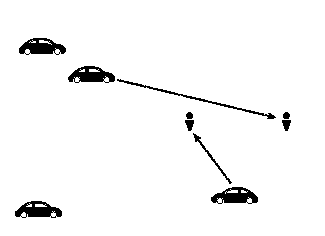
\includegraphics[width=\textwidth]{figures/RebalancingRedispatching1}
        \caption{Dispatching command with non-minimal summed pickup distance.}
        \label{fig:dispatch-subopt}
    \end{subfigure}
    ~ %add desired spacing between images, e. g. ~, \quad, \qquad, \hfill etc.
      %(or a blank line to force the subfigure onto a new line)
    \begin{subfigure}[b]{0.3\textwidth}
        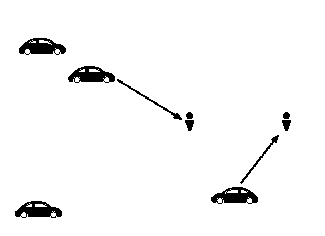
\includegraphics[width=\textwidth]{figures/RebalancingRedispatching2}
        \caption{Dispatching command with minimal summed pickup distance.}
        \label{fig:dispatch-opt}
    \end{subfigure}
    ~ %add desired spacing between images, e. g. ~, \quad, \qquad, \hfill etc.
    %(or a blank line to force the subfigure onto a new line)
    \begin{subfigure}[b]{0.3\textwidth}
        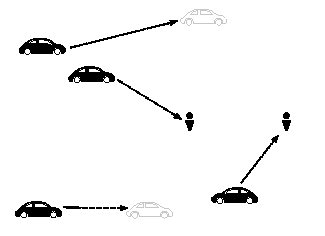
\includegraphics[width=\textwidth]{figures/RebalancingRedispatching3}
        \caption{Dispatching command with minimal summed pickup distance and rebalancing.}
        \label{fig:dispatch-optreb}
    \end{subfigure}
    \caption{Dispatching and Rebalancing Strategies}\label{fig:animals}
\end{figure}


Furthermore there is a charging and service process for the vehicles that influences the operational performance as well as parameters not related to the operation of vehicles (e.g. cleaning, interior design,...).

As there is a complex interaction between the fleet size, the amount of rebalancing, the operational strategies (dispatching and rebalancing), the service level and the costs for the operator, in \ref{subsec:performancemeasures} we propose what variables and charts to analyze to analyze the performance for AMoD systems.



\subsection{Performance of Autonomous Mobility on Demand Systems}
\label{subsec:performancemeasures}

The service level is mainly dependant on the customer wait times. We define the wait time as the time from the arrival of a taxi request to the system until an available vehicle has reached the spot. For a given fleet size, the distribution of wait times is analyzed for every time step of the day (see XYZ include figure). Furthermore the waiting time has to be analyzed as a function of the fleet size $N$, see e.g. XYZ include figure.

The operational cost that can be influenced with the choice of the operating strategy is mainly based on the driven distance. We distinguish three types of distances. Vehicles can either drive to pickup a customer, they can drive to rebalance or they can drive with a customer. Assuming a pricing scheme where customers pay for distance driven and time spent in the vehicle, the distance driven with customers can be assumed to be profitable distance. Furthermore the total distance driven with customers is contant when considering a fixed set of customer requests and assuming that vehicles travel the minimum distance path for each request in the network.

Thus the goal of each operational strategy is to minimize the total empty distance (pickup and rebalancing) by the vehicles. As shown in \cite{treleaven2011asymptotically} this distance cannot be driven to zero for general demand patterns, it is bounded below by the earth mover's distance which is a measure of how different the distribution of origins and destinations are in each time step, see e.g. \cite{ruschendorf1985wasserstein}. The earth mover's distance for the Zurich scenario considered in this work calculated for hourly time bins is shown in figure \ref{fig:EMD}.


\begin{figure}[h]
\begin{center}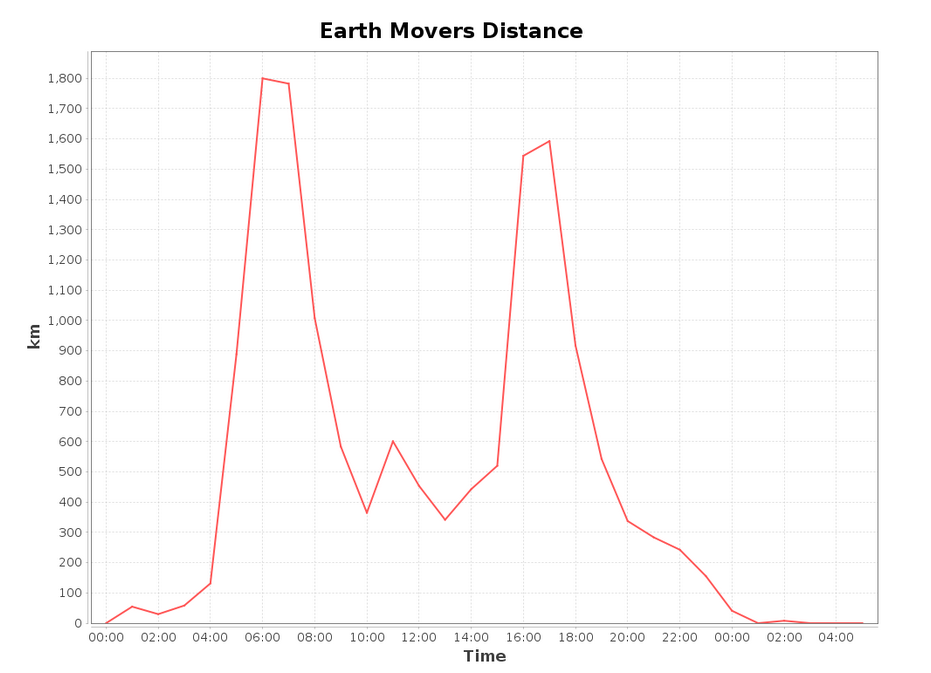
\includegraphics[width=0.9\textwidth]{figures/EMDZurich.png}\end{center}
\caption{Earth mover's distance for Zurich calculated for hourly time bins. XYZ make figure nicer.}
\label{fig:EMD}
\end{figure}

While the total amount of empty distance driven can not be reduced to zero, the ratio of pickup and rebalance distance driven can be influenced by the controller. A well-performing fleet controller will reposition vehicles already before the demand appears, i.e. it will increase the rebalance distance but reduce the pickup distance. Perfect estimation of future demands would lead to a system where almost all of the empty distance is rebalance distance. In order to make these concepts visible, we propose the plot in figure \ref{fig:study_area_vnodes} to assess the operational quality of an AMoD system. Distances that are profitable and cannot be avoided are plotted on the negative ordinate and empty distances on the positive ordinate. Furthermore the empty distances are distinguished into rebalancing and pickup distances. Any controller tries to minimize the area above the abscissa, ensure it is composed mostly of rebalancing distances and satisfy certain service level constraints.



\begin{figure}[h]
\begin{center}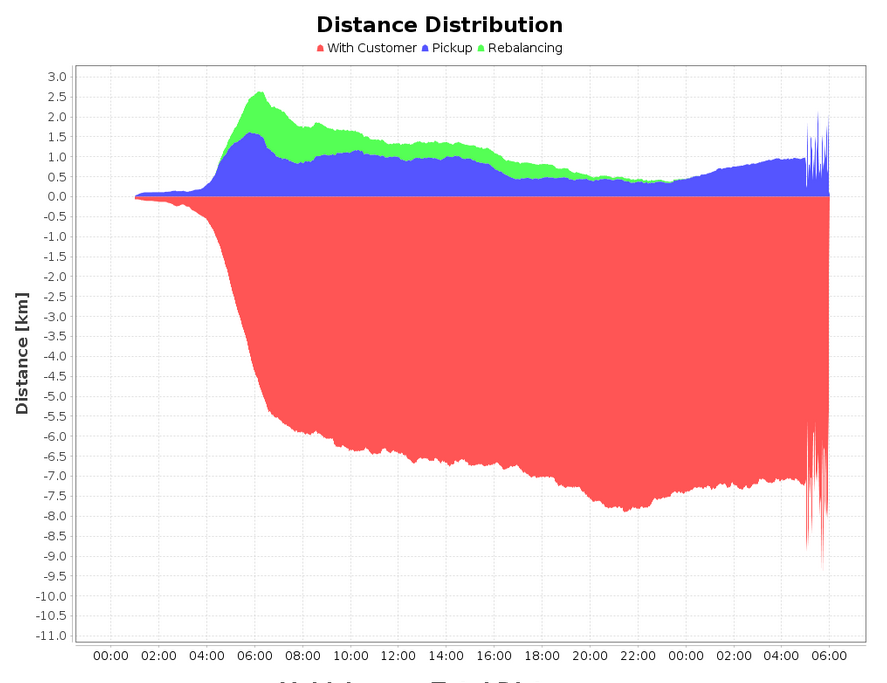
\includegraphics[width=0.9\textwidth]{figures/distancePlot.png}\end{center}
\caption{Distances with customer, pickup distances and rebalancing distances driven by the fleet in every time step. INCLUDE ANOTHER FIGURE or refence to actual figure shown in simulations XZY}
\label{fig:study_area_vnodes}
\end{figure}




\subsection{Automatic Control of Autonomous Mobility on Demand Systems}
\label{subsec:automaticControl}

In this work we analyze four different operating strategies from literature for the Zurich scenario, which are briefly outlined below:

\begin{enumerate}
\item The single heuristic dispatcher is the strategy presented in \cite{bischoff2016simulation}. In every dispatching time step $\delta t_D$ If there are more available vehicles than requests, it iterates on the list of requests and assigns to each request the closest vehicle. If there are more open requests than available vehicles, the controller iterates on the available vehicles and assigns the closest open request to each vehicle. The assignments are binding, i.e. they are not reopened once concluded.
\item The global Euclidean bipartite matching dispatcher determines an optimal bipartite matching between all open requests and available vehicles in every dispatching time step $\delta t_D$. The used distance function is the Euclidean distance which allows to use fast algorithms, e.g. \cite{agarwal2004near}. In contrast to the previous strategy, the assignments can be changed until a vehicle actually reaches its target. If arrival probabilties for future time steps is taken into account, this strategy can be considered as the optimal dispatching strategy based on Euclidean distances.
\item In \cite{pavone2011load} a feedforward strategy is presented on how to rebalance vehicles between different vertices in a directed graph $G = (V,E)$. For each vertex $i$ and time step $\delta_t$, the arrival rates $\lambda_i$ and transition probabilities $p_{ij}$ for any nodes $v_i, v_j \in V$  are used in a linear program to compute the optimal rebalancing flows $\alpha _{ij}$ in that time step assuming that the system is at equilibrium. To implement this strategy, we divided the city of Zurich into a set of areas. The nodes from \cite{pavone2011load} represent the centroids of these areas on which a complete directed graph called virtual network is placed, see figure \ref{fig:virtualNetwork}. Available cars are continuously rebalanced between the vertices of the virtual network according to the static rebalancing rates $\alpha_{ij}$. As the work does not detail the proposed dispatching algorithm for this strategy, we match cares using global Euclidean bipartite matching. Rebalancing vehicles cannot be dispatched until they reach their destination.
\item The last implemented strategy is as well derived from \cite{pavone2011load}. Instead of a pure feedforward solution, here in every rebalancing timestep $\delta t_R$ for every area of the virtual network the avaialble cars and open requests are counted and fed into an integer linear program which calculates the number of cars $reb _{ij}$ to be sent from virtual vertex $i$ to virtual vertex $j$. As in the feedforward strategy, the matching of the cars is done via global Euclidean bipartite matching.
\end{enumerate}



\begin{figure}[h]
\begin{center}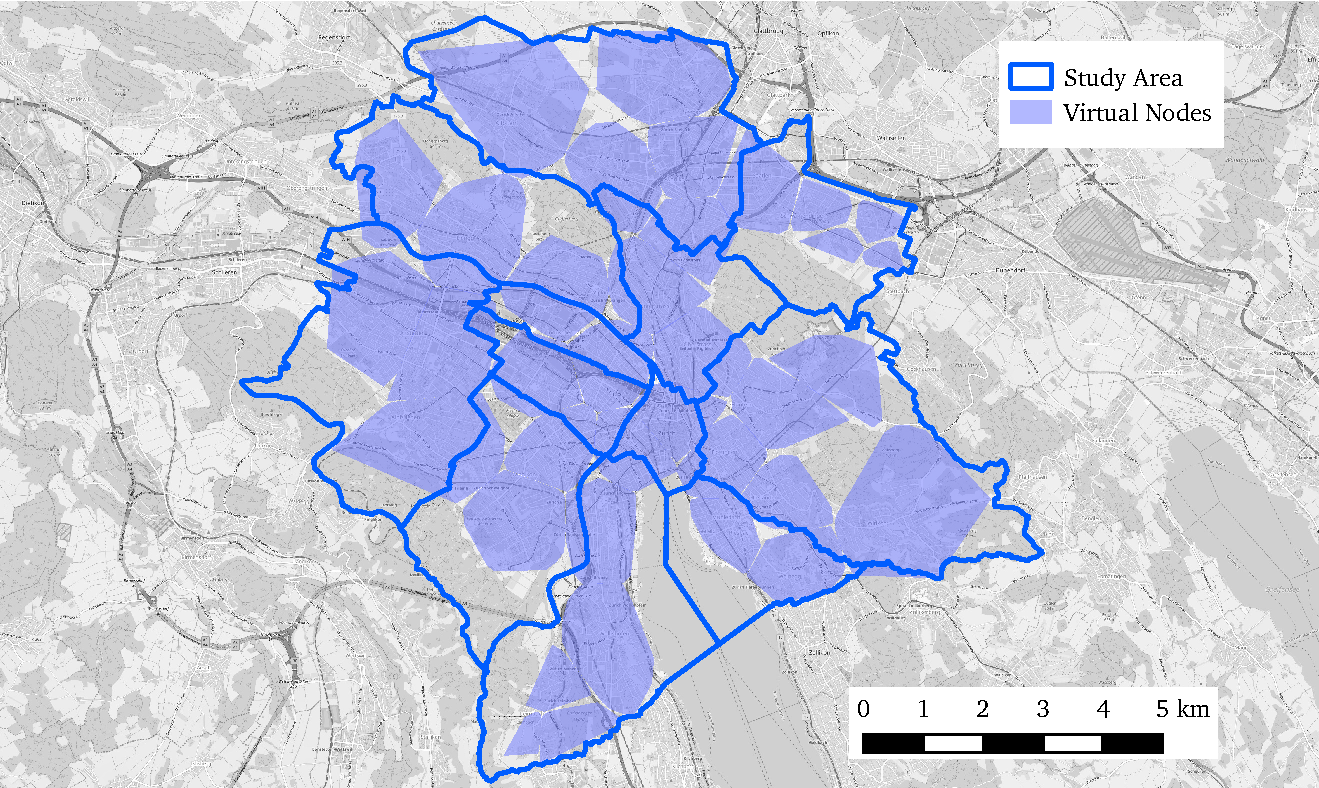
\includegraphics[width=1.0\textwidth]{figures/map.pdf}\end{center}
\caption{The study area covering the 12 districts of Zurich and the nodes of the virtual network for the rebalancing algorithms.}
\label{fig:study_area_vnodes}
\end{figure}

\subsection{Fleet sizing for Zurich}
\label{subsec:fleetSizing}

In this section we use strategies presented in \cite{spieser2014toward} to estimate the needed fleet size for a given scenario without actually using a simulation. We then compare these values to the simulation results in section XZY.

We define an AMoD system to be stable if the number of open requests is bounded for all times. A necessary condition for this to hold is that the distance the vehicles can drive collectively is larger than the distance to be driven to satisfy new requests entering the system. For every time step $k = 0,1,2,...,T$ over the course of a simulation we can define these quantities as $N \cdot v_k$ and $ \lambda_k \cdot d_{av,k}$ respectively, where $v_k$ is the average vehicle speed in time step $k$, $\lambda_k$ the customer arrival rate in timestep $k$ and $d_{av,k}$ the average distance per request in timestep $k$. Summing over the day, rearranging and using the fact that the average distance per trip is composed of the actual trip distance and the earth mover's distance, we can state that

\begin{align}
N \geq \frac{\lambda_k \cdot (d_{OD,k} + d_{EMD,k} )}{v_k}
\end{align}

where $d_{OD,k}$ and $d_{EMD,k}$ are the averge driving distance per request and the average earth mover's distance per request in timestep $k$ respectively. The analysis conducted on the scneario data yields a minimum fleet size of XZY for Zurich.

This number presents a lower bound for the fleet size such that the system can be stable, however it does not show what fleet sizes are necessary for an acceptable level of service. In order to estimate this number we used the strategy presented in \cite{spieser2014toward} where data of the requests is used to compute the vehicle availabilities using mean value analysis in a closed Jackson network for different fleet sizes. The availability of a node is defined as the probability that there is at least one vehicle waiting at the node. Computing this quantity for every node of a virtual network for Zurich  XZY include information on timestep XZY and taking the average of all stations, we can generate the following figure:




\begin{figure}[h]
\begin{center}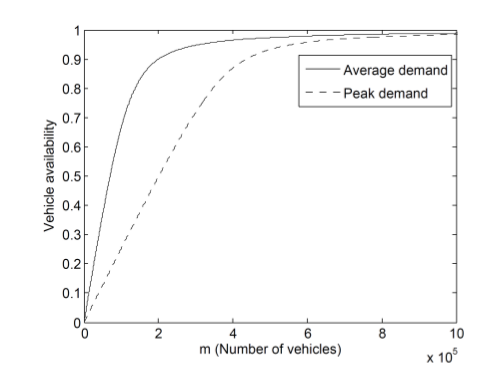
\includegraphics[width=0.9\textwidth]{figures/performancePlot.png}\end{center}
\caption{Performance driven fleet sizing for the city of Zurich according to \cite{spieser2014toward}. XZY put real plot}
\label{fig:performanceFleetSize}
\end{figure}

The results indicate that XZY include conclusion. XZY.

\section{Simulations}
\label{sec:staticSimulations}

The dispatching algorithms as presented before have been tested in the agent-
and activity-based transport simulation framework MATSim. What has been used in
this paper is the mobility simulation component of that package, where each agent
has a daily plan consisting of activities and legs. Activities are performed for a
certain duration at specific locations in the traffic network and have predefined
end times. They are connected by legs, which are performed by specific means of
transport. Dependent on the time of day, the mode, the route taken and other factors,
travel times may vary. Most importantly, the network is capacitated such that
congestion emerges if many agents use the same networks links at the same time.

Most important for the study at hand is the simulation of vehicles in an actual
network. By keeping background traffic in the simulation, the AVs are constrained
by the network conditions, most remarkably they suffer from longer travel times
at peak hours due to congestion.

The section is divided into two parts: First, we describe how the simulation
scenario has been set up to account for a realistic travel demand for Zurich.
Second, the simulation approach for automated vehicles is explained and third,
the results for the different dispatching algorithms are presented.

\subsection{Scenario Setup}
\label{sec:simulations_scenario}

For Switzerland the Microcensus on mobility and transport \cite{microcensus} is
available, which features the daily travel patterns of 60,000 Swiss residents.
In a previous study it has been used to create a detailed agent population of
Switzerland, which reproduces the demographic attributes and travel patterns
in the country to great detail \cite{ivtbaseline}.

Additional modifications have been applied to this population of around 8 million
agents to make it suitable for the study at hand. First, a best-response routing
of the travels of all agents has been performed to find all agents that interfere
with the study area, which has been defined to the 12 districts of Zurich (Figure \ref{fig:study_area_vnodes}).
All agents which do not interact with that region (performing an activity within
the area or crossing the area) have been deleted from the population as they do
not contribute to the state of the traffic system in that area. Finally, a 1\%
sample of the remaining agents has been created, which is the basis for our
simulations to account for feasible computation times for the proposed dispatching
algorithms.

In order to define the travel demand for the fleet of automated vehicles, agents
have been tagged as whether they are viable for using an automated vehicle or not.
While pedestrians and cyclists have not been simulated at all (since they do not
contribute to congestion in the current version of the framework), agents that
travel by car or public transit at least once during their daily plan are
handled differently.

Agents that travel at least once by private car during the simulation are tagged
as an AV user \textit{only} if all of the legs in the agent's plan take place
within the study area. This constraint makes sure that no unrealistic travel
plans are generated, where an agent performs his first leg by AV although his
private car is at home and then wants to depart at the next location with that
car. Finally, the ``car'' legs of all viable have been converted to the ``av'' mode.
All other legs are kept as before, i.e. short legs that were assigned the ``walk''
mode before are still performed in this mode.

For agents that use public transit, the procedure is different. Here, any leg
that is performed by the ``pt'' mode in the original population is converted to ``av''
if it lies within the study area of 15km. As for car users, connecting non-motorized
legs are kept fixed.

This way a demand for Zurich has been generated where each leg that possibly
\textit{can} be performed using an AV \textit{is} using an AV. In that sense we
simulate a scenario where 100\% of the AV travel demand must be served by the
dispatchers.

To summarize, the 8,230,971 agents in the population have been decimated to
1,935,400 agents, which interfere with the study area. From this set of agents
a 1\% sample has is drawn, leading to 19,354 agents that mainly constitute
background traffic. Among those are 970 agents that are viable for the AV
service. The plans of these agents contain 4030 trips that are to be served by
AVs. In reality, this service would hence need to serve 403,000 requests by
97,000 persons.

\subsection{Simulation of automated vehicles}

To simulate automated vehicles in the MATSim scenario, a framework extension by
Hörl \cite{horl_abmtrans17} is used. There, AVs are individually simulated on the
road network, contributing to and experiencing congestion. As soon as agents
finish their activities the simulation is notified about an incoming request
given that the agent wishes to use an AV for the following leg. In that case
the request with its properties (departure time, origin, destination) is passed
on to the dispatcher. These dispatchers are based on different algorithms, as
described before. However, the ``lifecycle'' of a request is always the same: First,
an AV needs to drive to the location of the customer, pick him up, drive to the
final location and finally drop the customer off. From the point a customer has
been picked up, the process is predetermined, no changes to the route of the AV
are made anymore. While an AV has been assigned to a customer for pickup the
vehicle may be reassigned depending on the dispatching algorithm.

It should be noted that AVs drive directly to the locations where agents end and
start their activities. So far no mechanism is implemented that would allow them
to meet at optimized locations (e.g. a high-capacity avenue instead of a small
alley).

\section{Results}
\label{sec:results}

We test the four proposed dispatching strategies in the Zurich scenario with four
runs per strategy. Each run simulates 20 iterations to allow the dispatchers to sense
the traffic conditions in the network, i.e. to figure out what travel times on
specific links are expected and how traffic jams can be avoided.

For Zurich, the times with peak congestion and, hence, longest travel times are
from 6:30am to 9:00am and from 4:30pm to 6:30pm. In figure \ref{fig:mean_peak_waiting_times}
all trips by AV with departures times in these time windows are collected
and the mean waiting time for vehicle is computed. As expected, the average
waiting time is decreasing with larger fleet sizes and higher availabiltiy of
vehicles. Almost over the whole range of flet sizes the feedback LP dispatcher
performs best, while the load-balancing heuristic features the longest waiting
times.

\begin{figure}
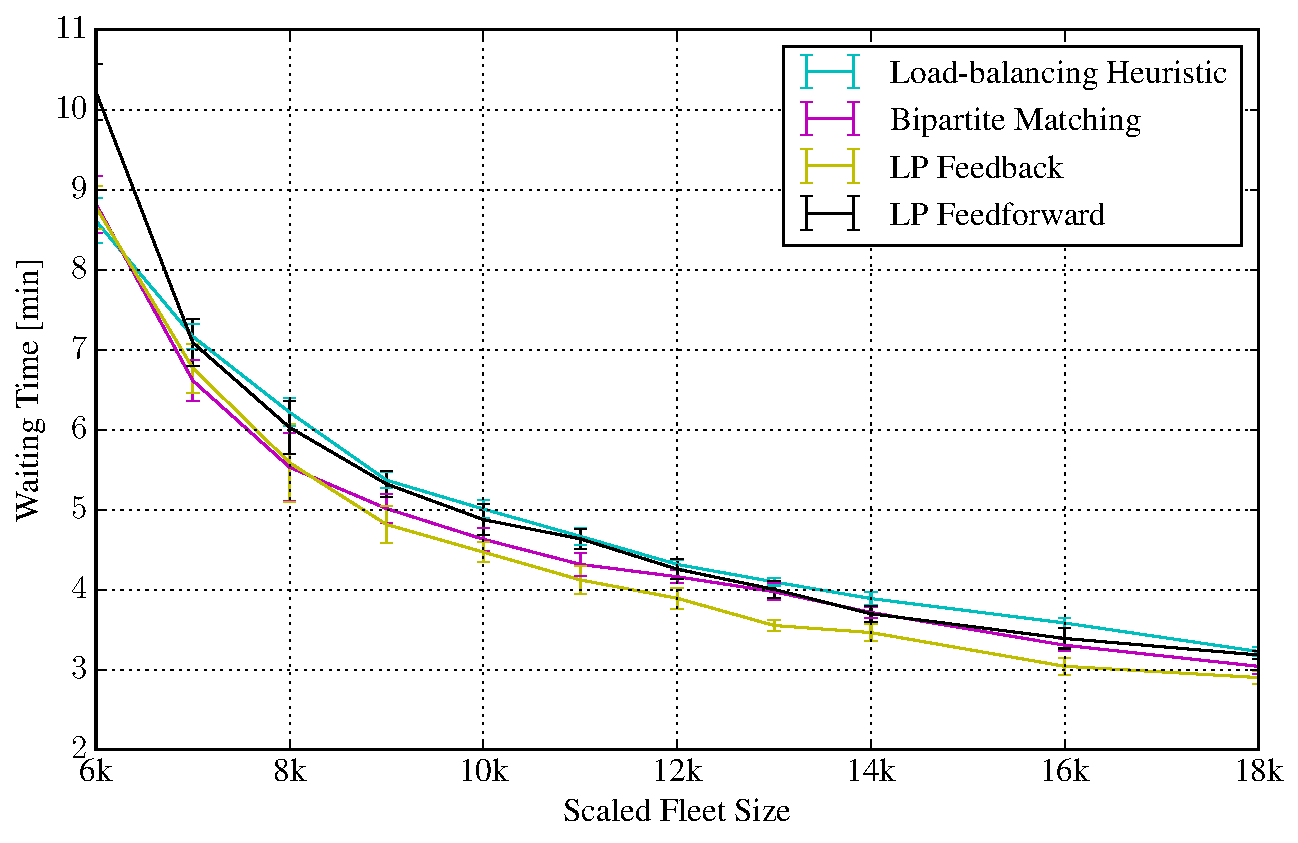
\includegraphics[width=1.0\textwidth]{figures/mean_peak_waiting_times.pdf}
\caption{Average waiting time for an AV to arrive at peak times}
\label{fig:mean_peak_waiting_times}
\end{figure}

Figure \ref{fig:empty_rides} shows the percentage of fleet mileage that is driven
without a customer, either for pickup or rebalancing purposes. Clearly, the LP
algorithms, which both use rebalancing, have a higher share of empty mileage
that the non-rebalancing approaches. The heuristic approach manages to keep the
share lowest, since it mainly operates in a best-response state, where only the
shortest pickup trips are chosen. Remarkably, the total driven distance for all
dispatchers is very similar (Figure \ref{fig:total_distance}), which indicates
that the surplus of empty distance for the intelligent dispatchers does not stem
from inefficient movements, but rather effective movements towards the expected
customer demand for shorter waiting times.

[TODO: Do we need two plots here? Also a plot Total Distance <-> Relative Distance
would be possible, where one can traverse the fleet size along the graph]

\begin{figure}
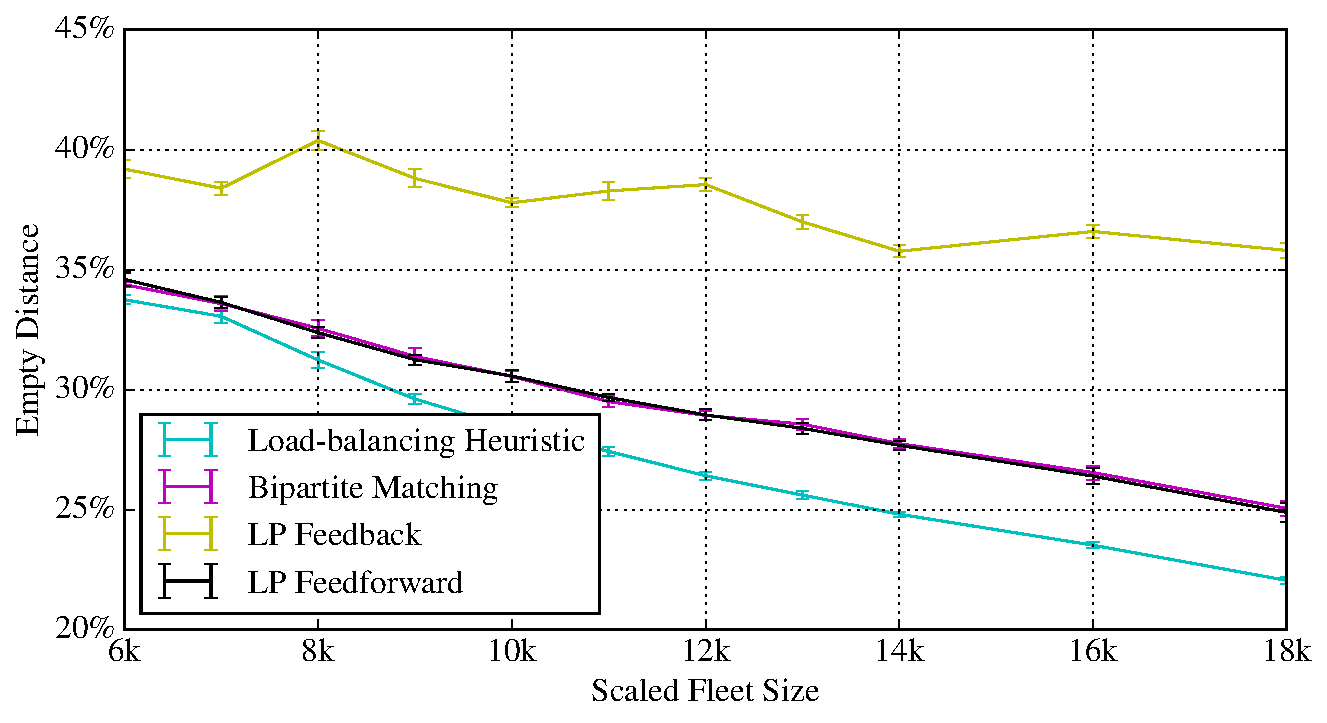
\includegraphics[width=1.0\textwidth]{figures/empty_rides.pdf}
\caption{The fraction of distance that is driven by AVs without a passenger.}
\label{fig:empty_rides}
\end{figure}

\begin{figure}
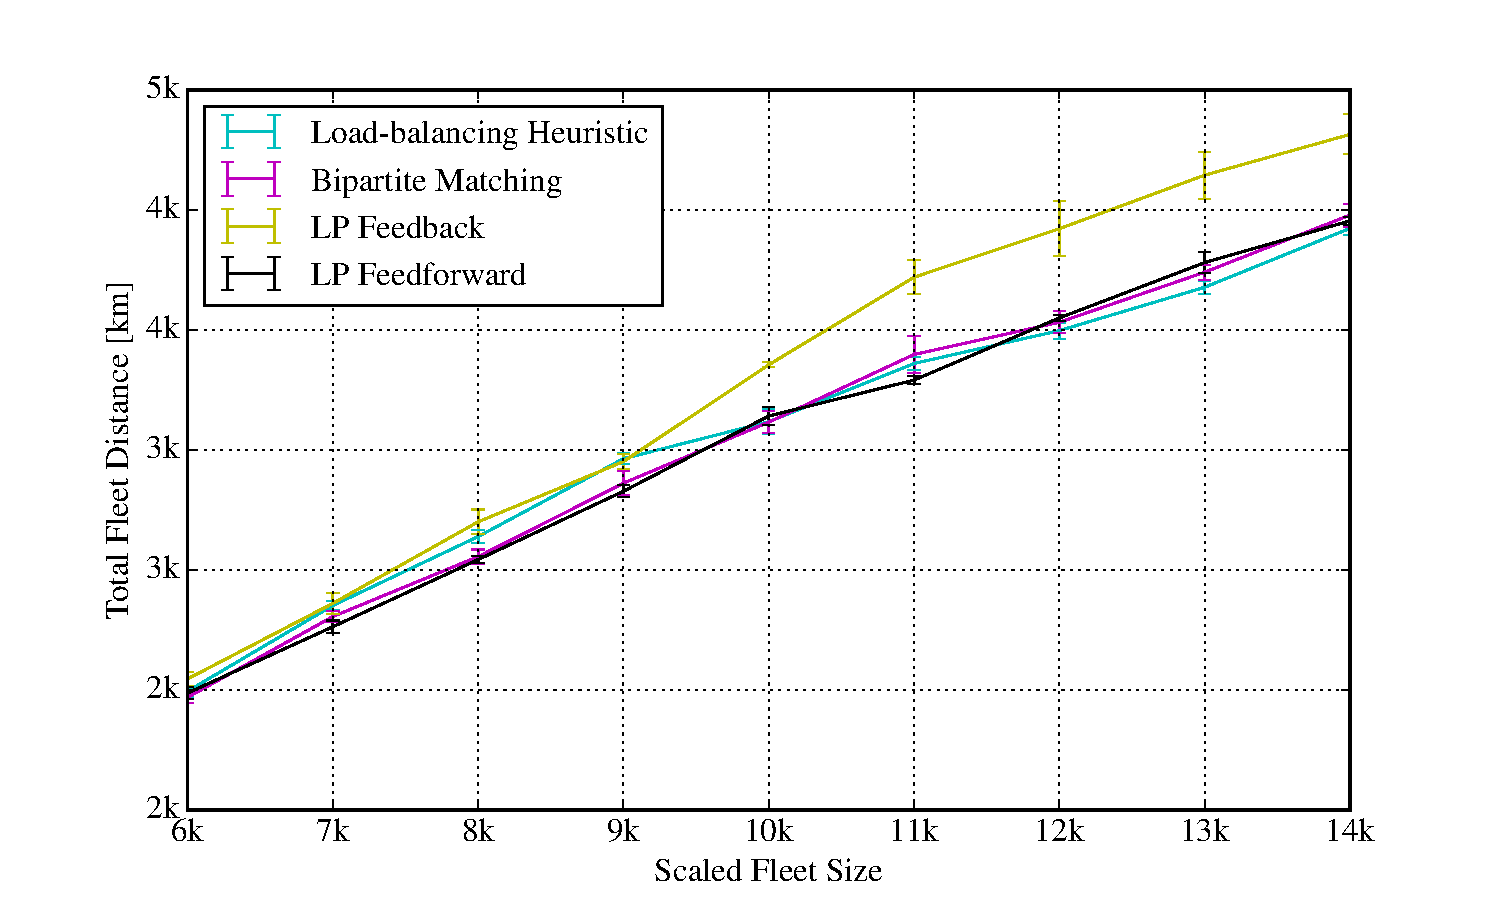
\includegraphics[width=1.0\textwidth]{figures/total_distance.pdf}
\caption{The total distance that is driven by AVs, with and without passenger on-board.}
\label{fig:total_distance}
\end{figure}

Finally, figure \ref{fig:occupancy} shows the occupancy of the fleet for different
fleet sizes. Since in the 30h MATSim simulation no AV trips are registered in
the hours around midnight, it is possible to correct the resulting 30h occupancy
rate to one that is based on a 24h day. As can be seen, the occupancy of all
fleet dispatchers exceeds the 8\% that is common today. In general, one can say
that the dispatching algorithm has only little influence on fleet occupancy. The
differences lie in the range of 0.5\% between the best and worst performing algorithm,
which are the LP Feedback dispatcher and the load-balancing heuristic, respectively.
Nevertheless, one can see that the occupancy of the latter is systematically lowest.

\begin{figure}
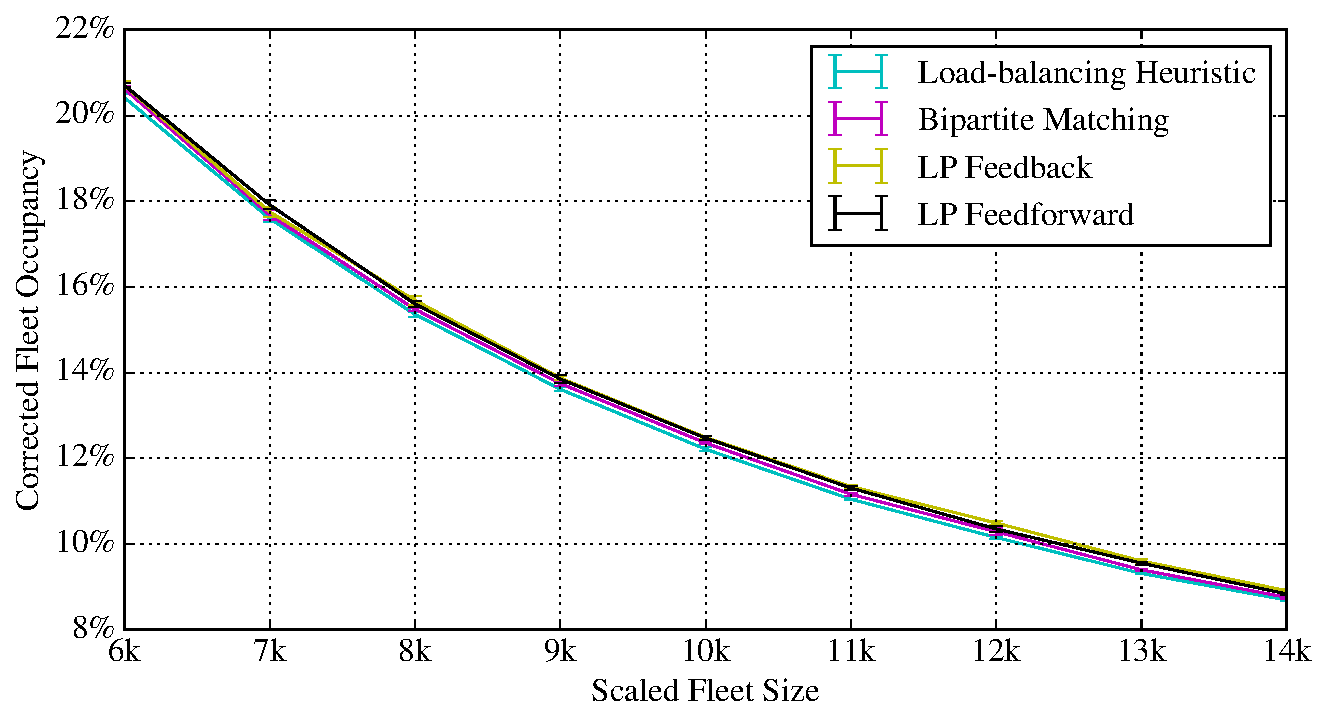
\includegraphics[width=1.0\textwidth]{figures/occupancy.pdf}
\caption{The occupancy of the AV fleet for different flet sizes.}
\label{fig:occupancy}
\end{figure}

\subsection{Cost Analysis}
\label{sec:cost_analysis}

Based on a paper Bösch et al. \cite{cost_paper} the costs of operating the simulated
AV services are computed. Specifically, by providing their calculator with key
figures of the operator (among them the occupancy, the share of empty rides, the
average travel distance) the price that the operator would at least need to ask
a customer per kilometer if a profit margin of at least 3\% is targeted. The calculation
is based on a detailed analysis of running and fixed costs. Figure~\ref{fig:passenger_price}
shows the results from this analysis. Unsurprisingly, the price that needs to be
imposed on the customer increases with larger fleet sizes. However, the increase
is stronger for the load-balancing heuristic than for any other distpaching strategy.
Therefore, with the same fleet being available to an operator, he would be able
to offer the service for almost 0.10 CHF less per kilometer than before or save
this amount of money.

\begin{figure}
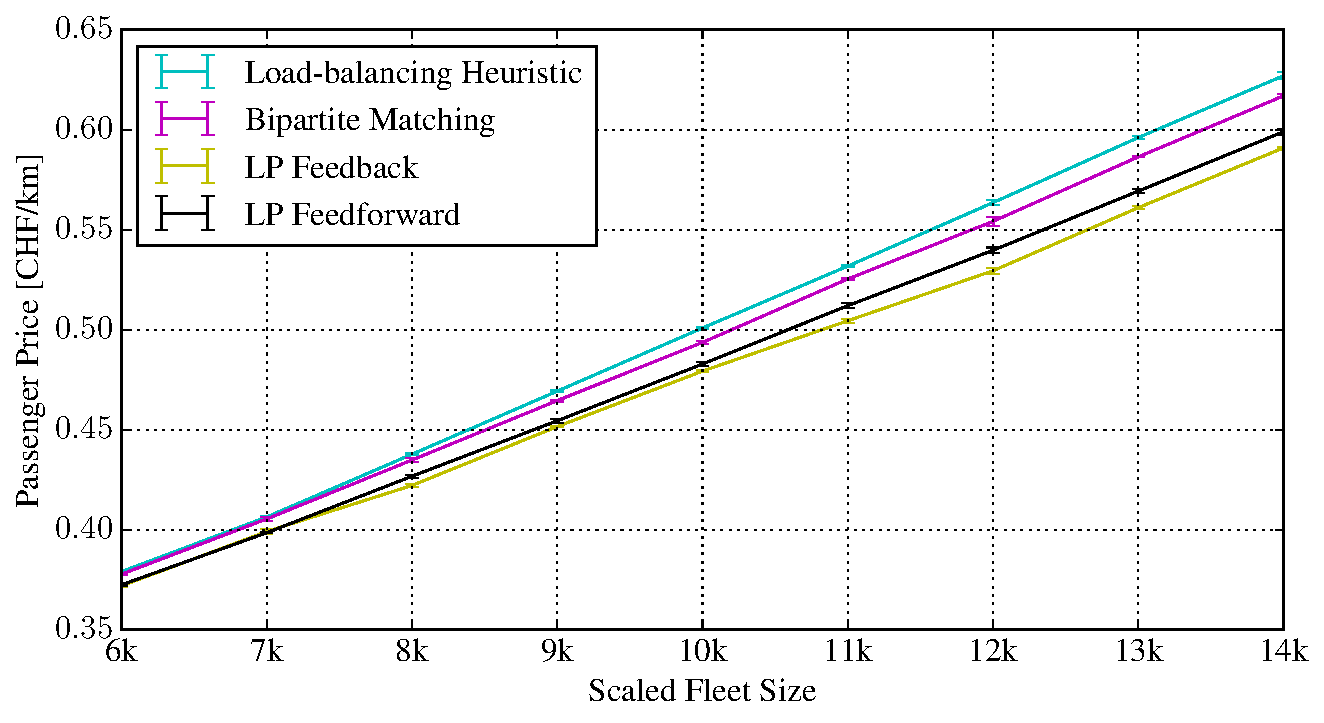
\includegraphics[width=1.0\textwidth]{figures/01_passenger_price.pdf}
\caption{The minimum customer prices that an AV operator needs to charge the customer
in order to have a win margin of at least 3\%.}
\label{fig:passenger_price}
\end{figure}

Compared to the average running costs of driving a private car in Switzerland
(around 0.17 CHF/km) or using public transit (around 0.25 CHF/km) [TODO CITATIONS]
the computed prices still seem rather high. Compared to conventional taxi operators,
however, the price is extremely low (around 6 CHF/km). Therefore, it is imaginable
that the AV service would still be attractive for a large group of people, for
which a conventional taxi would be too expensive on a daily basis, but an AV would
make such travels affordable.

However, the attractiveness of an AV service does not only depend the price itself,
but also on the attitudes of the people towards the service. One key component to
the acceptance of an AMoD system is the waiting times that customers need to endure.
Figure \ref{fig:time_vs_price} combines the key results from our simulations. There,
the price that a specific operator configuration (fleet size and dispatcher) is
displayed in comparison to the waiting time that this operator can offer.
Assuming that, for instance, a waiting time of five minutes is tolerable, the
operator could offer a satisfactory service for around 0.45 CHF with the feedback
dispatcher, while he would need to charge 0.50 CHF with the simple load-balancing
heuristic. The better the level of service of the operator is ought to be, the larger
this margin becomes.

\begin{figure}
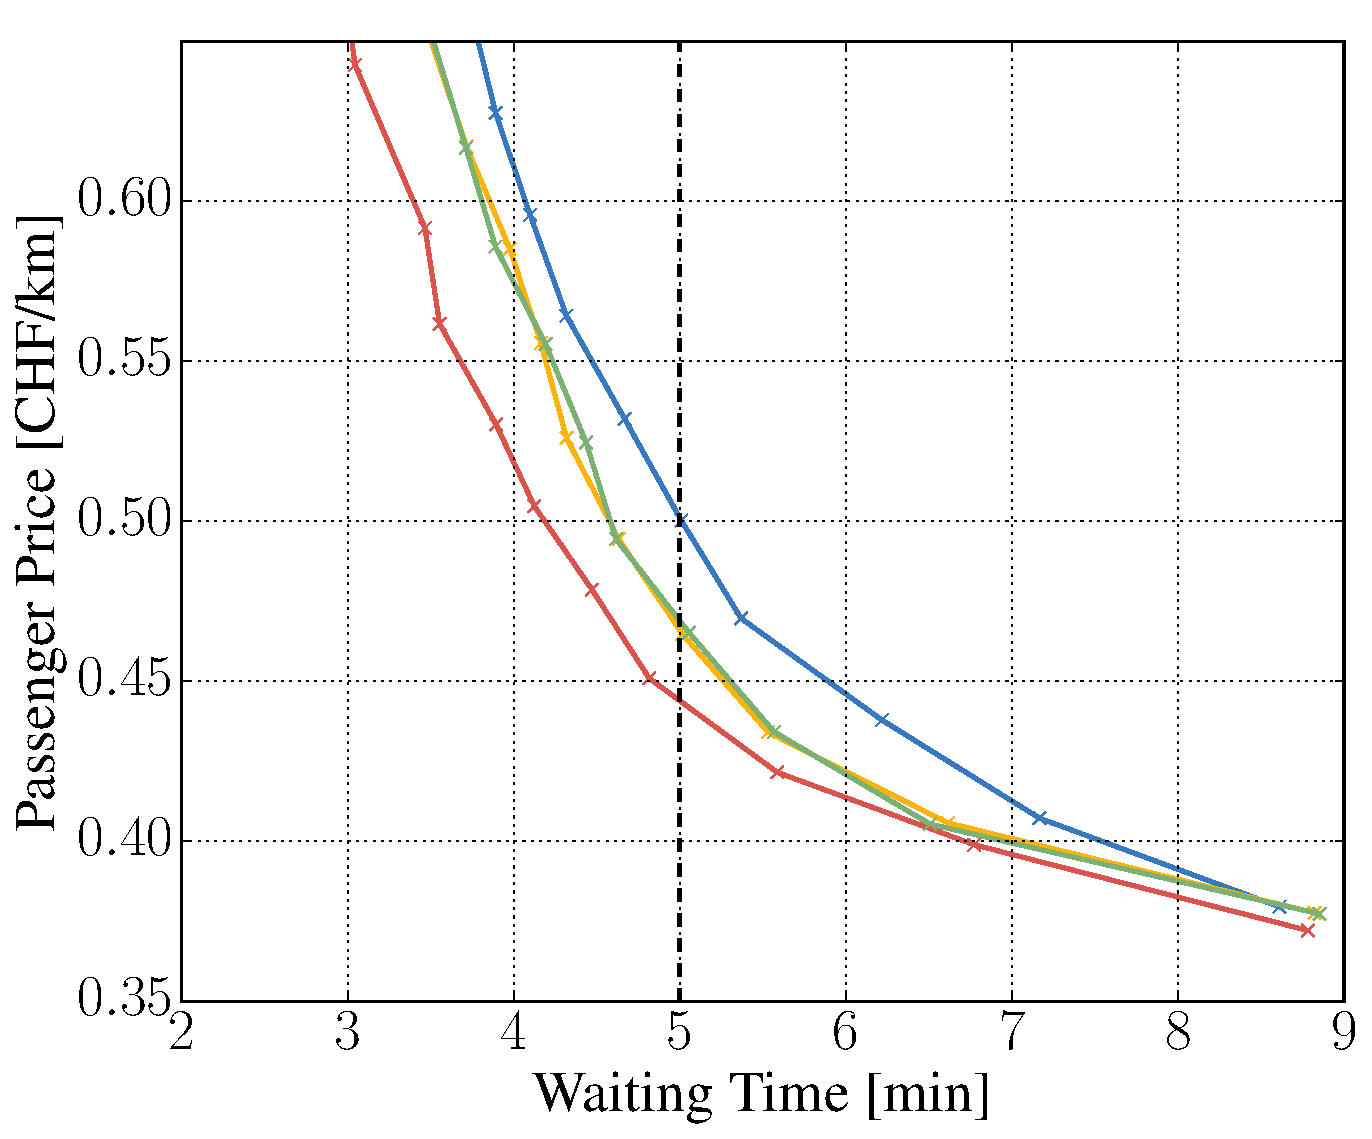
\includegraphics[width=1.0\textwidth]{figures/time_vs_price.pdf}
\caption{Time vs. Price}
\label{fig:time_vs_price}
\end{figure}

\section{Discussion \& Conclusion}
\label{sec:Conclusion}

The study shows that the right choice of dispatching algorithm for an AMoD system
does not only have strong impact on the performance in terms of waiting times for
the customer, but also that it bears a significant economic advantage for the
operator. He is able to attract more customers through quicker pickups and
lower prices than a competitor with only little investment.

In order to assess the significance for real fleets of (not neccessarily
automated) taxis it needs to be noted that all of the presented algorithms are
able to process dispatching and rebalancing tasks for fleets of thousands of
vehicles within minutes. It is perfectly feasible to control 100k vehicles in
five minute updates using a standard laptop for the computational tasks.

For the presented simulations, this still poses a burden, though, because there
a speedup compared to reality of around one thousand times is desired to be able
to run large numbers of simulations with different parameters. Hence, the algorithms
could only be tested on a subsample of 1\% of the agent population that is available.

[ TODO: OTHER LIMITATIONS ]


%\input{Background}
%\input{ScoringMATSim}
%\input{ProposedScoringFunction}
%\input{DefaultProposedUtilityFunction}
%\input{ReschedulingResults}
%\input{Discussion}
%\input{Conclusion}
%%%%%%%%%%%%%%%%%%%%%%%%%%%%%%%%%%%%%%%%%%%%%%%%%%%%%%%%%%%%%%%%%%%%%%
%% Bibliography
%%   Leave this as is, and add you own entries to my.bib
%%   Many references are already defined in _latexfiles/bibs/all-eng.bib
%%   Refer to the BibTeX/LaTeX tutorial for adding new entries
%%   to the IVT BibTeX database
\bibliography{\mypath/bibs/all-eng,my}
%%%%%%%%%%%%%%%%%%%%%%%%%%%%%%%%%%%%%%%%%%%%%%%%%%%%%%%%%%%%%%%%%%%%%%

%%%%%%%%%%%%%%%%%%%%%%%%%%%%%%%%%%%%%%%%%%%%%%%%%%%%%%%%%%%%%%%%%%%%%%
%% Appendices
%%   Usually they would start on a separate page
%%%%%%%%%%%%%%%%%%%%%%%%%%%%%%%%%%%%%%%%%%%%%%%%%%%%%%%%%%%%%%%%%%%%%%


\end{document}

%%%%%%%%%%%%%%%%%%%%%%%%%%%%%%%%%%%%%%%%%%%%%%%%%%%%%%%%%%%%%%%%%%%%%%
%%%%%%%%%%%%%%%%%%%%%%%%%%%%%%%%%%%%%%%%%%%%%%%%%%%%%%%%%%%%%%%%%%%%%%
%%
%% END OF DOCUMENT
%%
%%%%%%%%%%%%%%%%%%%%%%%%%%%%%%%%%%%%%%%%%%%%%%%%%%%%%%%%%%%%%%%%%%%%%%
%%%%%%%%%%%%%%%%%%%%%%%%%%%%%%%%%%%%%%%%%%%%%%%%%%%%%%%%%%%%%%%%%%%%%%

%%%%%%%%%%%%%%%%%%%%%%%%%%%%%%%%%%%%%%%%%%%%%%%%%%%%%%%%%%%%%%%%%%%%%%
%% Editor specific keywords:
%%   This is not part of you paper, but sometimes it is used
%%   for additional features of TeX Editors.
%%
%% WinEdt:
%%   to get the bibliography list
%GATHER{./_bibs/all-eng.bib}
